\documentclass[lang=cn,10pt]{elegantbook}

\usepackage{url}

\title{\LaTeX{} 2639002.01 LTC8631实验报告}
% \subtitle{Elegant\LaTeX{} 经典之作}

\author{}
\institute{Elegant\LaTeX{} Program}
\date{\zhtoday}
\version{4.3}

\extrainfo{不要以为抹消过去,重新来过,即可发生什么改变。—— 比企谷八幡}

\setcounter{tocdepth}{3}

\logo{logo-blue.png}
\cover{cover.jpg}

% 本文档命令
\usepackage{array}
\newcommand{\ccr}[1]{\makecell{{\color{#1}\rule{1cm}{1cm}}}}

% 额外package
\usepackage{xeCJK} % 在公式里输入中文
\xeCJKsetup{CJKmath=true} % 在公式里输入中文
\usepackage[makeroom]{cancel} % 删去符号,X

% 修改标题页的橙色带
\definecolor{customcolor}{RGB}{32,178,170}
\colorlet{coverlinecolor}{customcolor}

\def\0{{\mathbf 0}}
\def\1{{\mathbf 1}}

\def\a{{\mathbf a}}
\def\b{{\mathbf b}}
\def\c{{\mathbf c}}
\def\d{{\mathbf d}}
\def\e{{\mathbf e}}
\def\f{{\mathbf f}}
\def\g{{\mathbf g}}
\def\h{{\mathbf h}}
\def\i{{\mathbf i}}
\def\j{{\mathbf j}}
\def\k{{\mathbf k}}
\def\l{{\mathbf l}}
\def\m{{\mathbf m}}
\def\n{{\mathbf n}}
\def\o{{\mathbf o}}
\def\p{{\mathbf p}}
\def\q{{\mathbf q}}
\def\r{{\mathbf r}}
\def\s{{\mathbf s}}
\def\t{{\mathbf t}}
\def\u{{\mathbf u}}
\def\v{{\mathbf v}}
\def\w{{\mathbf w}}
\def\x{{\mathbf x}}
\def\y{{\mathbf y}}
\def\z{{\mathbf z}}

\def\A{{\mathbf A}}
\def\B{{\mathbf B}}
\def\C{{\mathbf C}}
\def\D{{\mathbf D}}
\def\E{{\mathbf E}}
\def\F{{\mathbf F}}
\def\G{{\mathbf G}}
\def\F{{\mathbf F}}
\def\H{{\mathbf H}}
\def\I{{\mathbf I}}
\def\J{{\mathbf J}}
\def\K{{\mathbf K}}
\def\L{{\mathbf L}}
\def\M{{\mathbf M}}
\def\N{{\mathbf N}}
\def\O{{\mathbf O}}
\def\P{{\mathbf P}}
\def\Q{{\mathbf Q}}
\def\R{{\mathbf R}}
\def\S{{\mathbf S}}
\def\T{{\mathbf T}}
\def\U{{\mathbf U}}
\def\V{{\mathbf V}}
\def\W{{\mathbf W}}
\def\X{{\mathbf X}}
\def\Y{{\mathbf Y}}
\def\Z{{\mathbf Z}}


\def\rE{{\text{E}}}
\def\rPr{{\text{Pr}}}
\def\Tr{{\text{Tr}}}
% \def\vec{{\textbf{}}}
\def\ie{{\textit{i.e.}}}
\def\eg{{\textit{e.g.}}}


\def\cA{{\mathcal A}}
\def\cB{{\mathcal B}}
\def\cC{{\mathcal C}}
\def\cD{{\mathcal D}}
\def\cE{{\mathcal E}}
\def\cF{{\mathcal F}}
\def\cG{{\mathcal G}}
\def\cH{{\mathcal H}}
\def\cI{{\mathcal I}}
\def\cK{{\mathcal K}}
\def\cL{{\mathcal L}}
\def\cM{{\mathcal M}}
\def\cN{{\mathcal N}}
\def\cO{{\mathcal O}}
\def\cP{{\mathcal P}}
\def\cQ{{\mathcal Q}}
\def\cR{{\mathcal R}}
\def\cS{{\mathcal S}}
\def\cT{{\mathcal T}}
\def\cU{{\mathcal U}}
\def\cV{{\mathcal V}}
\def\cW{{\mathcal W}}
\def\cX{{\mathcal X}}
\def\cY{{\mathcal Y}}
\def\cZ{{\mathcal Z}}


\def\bphi{{\pmb{\phi}}}
\def\bpsi{{\pmb{\psi}}}
\def\bphi{{\pmb{\phi}}}
\def\bpsi{{\pmb{\psi}}}
\def\balpha{{\boldsymbol \alpha}}
\def\bbeta{{\boldsymbol \beta}}
\def\bvarphi{{\boldsymbol \varphi}}
\def\bPhi{{\boldsymbol \Phi}}


\def\bcdot{{\;\boldsymbol{\cdot}\;}}

\def\ie{{\textit{i.e.}}}
\def\eg{{\textit{e.g.}}}

\begin{document}

\maketitle
\frontmatter

\tableofcontents

\mainmatter

\chapter{摘要}

本实验报告利用 LTspice 对 LT8631 进行了全面而深入的仿真分析。仿真测试了 LT8631 在不同输出电压条
件下的效率曲线、突发模式波形、开关模式波形、负载瞬态响应、输入电压瞬态响应以及启动失调电压性能等。
通过对比仿真结果与数据手册,验证了 LT8631 的各项指标和性能参数。
在仿真过程中运用了 LTspice 的各种测量和分析命令,如 .STEP、.TRAN、.MEAS 等,并熟练掌握了波形
查看器的操作方法。遇到的问题也都通过查阅资料、分析电路原理得以有效解决。
本次 LTspice 仿真实验,不仅检验了 LT8631 的工作性能,也充分训练和提高了自身的仿真设计与分析能力,
为后续深入学习各类 DC/DC 转换器奠定了坚实的基础。总体而言,本次仿真实验取得了圆满的成果。

\textbf{关键词}: LT8631; LTspice; 仿真; 效率; 瞬态响应; LaTeX

\chapter{引言}

\section{产品介绍}

LT8631 是一款电流模式 PWM 降压 DC/DC 转换器,内置同步开关,可为最大 1A 的输出负载提供电流。
它的输入范围广泛,从 3V 到 100V,适用于从多种电源进行电力调节,包括汽车和工业系统以及 36V 到 72V 的电信电源。
它采用低纹波突发模式运行,能够在保证输出纹波低于 10mV P-P 的情况下,实现高效的微小输出电流运行。
它的频率范围可以通过电阻编程,从 100kHz 到 1MHz,并具有同步功能,可以在效率和外部元件大小之间进行优化。
它的软启动功能可以控制输出电压的上升速率,避免启动时产生输入电流冲击,同时还可以实现输出跟踪。
它有一个电源良好的指示信号,当输出电压在调节输出的 ±7.5\% 范围内时发出。
它的欠压锁定功能可以通过 EN/ UV 引脚进行设置。
它的关机模式可以将总静态电流降低到 < 5µA。
LT8631 采用 20 引脚 TSSOP 封装,带有散热垫,具有低热阻和高电压引线间距的特点。[1]

\section{相关产品}

以下是三款与 LT8631 相关的产品,以及它们与 LT8631 的优缺点对比:

\begin{table}[h]
\centering
\begin{tabular}{@{}llll@{}}
\toprule
型号 & 输出电流 & 静态电流 & 价格(美元) \\ \midrule
LTC3631 & 500mA & 12$\mu$A & 3.75 \\
LT8331 & 500mA & 6$\mu$A & 3.95 \\
LT8640 & 5A & 2.5$\mu$A & 5.95 \\ \bottomrule
\end{tabular}
\caption{与 LT8631 相关的产品的主要参数}
\label{tab:products}
\end{table}

\begin{itemize}
\item \href{https://www.analog.com/en/products/ltc3631.html}{LTC3631}:这是一款 150V、500mA 同步整流式降压型 DC/DC 转换器,具有内部同步开关,输入电压范围为 4.5V 到 150V,输出电压范围为 0.8V 到 30V。它的工作频率可以通过电阻编程,从 250kHz 到 1MHz,并具有同步功能。它的静态电流为 12$\mu$A,低于 LT8631 的 16$\mu$A。它的价格为 3.75 美元(每片,1000片起订)。
    \begin{itemize}
    \item 优点:输入电压范围更宽,静态电流更低,价格更便宜。
    \item 缺点:输出电流更小,输出电压范围更窄,最大占空比更低(90\% vs 99\%)。
    \end{itemize}
\item \href{https://www.analog.com/en/products/lt8331.html}{LT8331}:这是一款 140V、500mA 降压/升压 DC/DC 转换器,具有内部同步开关,输入电压范围为 3V 到 140V,输出电压范围为 1.25V 到 60V。它的工作频率可以通过电阻编程,从 100kHz 到 2MHz,并具有同步功能。它的静态电流为 6$\mu$A,远低于 LT8631 的 16$\mu$A。它的价格为 3.95 美元(每片,1000片起订)。
    \begin{itemize}
    \item 优点:输入电压范围更宽,静态电流更低,工作频率更高,可以实现降压或升压的转换。
    \item 缺点:输出电流更小,输出电压范围更窄,最大占空比更低(85\% vs 99\%)。
    \end{itemize}
\item \href{https://www.analog.com/en/products/lt8640.html}{LT8640}:这是一款 65V、5A 同步整流式降压型 DC/DC 转换器,具有内部同步开关,输入电压范围为 3.4V 到 65V,输出电压范围为 0.8V 到 18V。它的工作频率可以通过电阻编程,从 200kHz 到 3MHz,并具有同步功能。它的静态电流为 2.5$\mu$A,远低于 LT8631 的 16$\mu$A。它的价格为 5.95 美元(每片,1000片起订)。
    \begin{itemize}
    \item 优点:输出电流更大,静态电流更低,工作频率更高,效率更高(最高 96\% vs 93\%)。
    \item 缺点:输入电压范围更窄,输出电压范围更窄,价格更贵。
    \end{itemize}
\end{itemize}

综上所述,LT8631 的主要优势是具有高输出电流、宽输出电压范围和高最大占空比的特点,适合用于需要大电流和低压降的应用场合。它的主要缺点是静态电流较高,工作频率较低,效率较低。

\chapter{任务模块总览}

本任务的目标是使用LTspice,一款强大、快速、免费的SPICE仿真软件,对LT8631,一款100V,1A的同步微功耗降压型稳压器,进行各种工作条件下的性能分析。\cite{bworld}具体包括以下几个任务模块:

\begin{itemize}
    \item Efficiency at VOUT = 5V:该任务模块的功能是分析在输出电压为5V时,LT8631的效率随输入电压和负载电流的变化情况。可以通过设置输入电压和负载电流的范围,并使用.STEP命令进行重复分析,得到效率的曲线图。
    \item Efficiency at VOUT = 3.3V:该任务模块的功能是分析在输出电压为3.3V时,LT8631的效率随输入电压和负载电流的变化情况。方法同上,只需修改输出电压的值即可。
    \item Efficiency (SWITCHING FREQUENCY (kHz) 和 EFFICIENCY 的关系):该任务模块的功能是分析在不同的开关频率下,LT8631的效率如何变化。可以通过修改RT引脚的电阻值,来改变开关频率,并使用.STEP命令进行重复分析,得到效率的曲线图。
    \item Burst Waveforms ($V_{\text{IN}} = 12V$ LOAD = 5mA):该任务模块的功能是观察在输入电压为12V,负载电流为5mA时,LT8631的突发模式波形。可以通过使用.TRAN命令进行瞬态分析,并使用波形查看器来显示输出电压、开关电压、开关电流等信号的波形。
    \item Burst Waveforms 2 ($V_{\text{IN}} = 100V$ LOAD = 50mA):该任务模块的功能是观察在输入电压为100V,负载电流为50mA时,LT8631的突发模式波形。方法同上,只需修改输入电压和负载电流的值即可。
    \item Switching Waveforms ($V_{\text{IN}} = 12V$ LOAD = 5mA):该任务模块的功能是观察在输入电压为12V,负载电流为5mA时,LT8631的开关模式波形。可以通过使用.TRAN命令进行瞬态分析,并使用波形查看器来显示输出电压、开关电压、开关电流等信号的波形。
    \item Switching Waveforms 2 ($V_{\text{IN}} = 100V$ LOAD = 50mA):该任务模块的功能是观察在输入电压为100V,负载电流为50mA时,LT8631的开关模式波形。方法同上,只需修改输入电压和负载电流的值即可。
    \item Load Transient Response (200mA to 800mA LOAD TRANSIENT $V_{\text{IN}} = 15V$):该任务模块的功能是观察在输入电压为15V时,LT8631的负载瞬态响应。可以通过使用一个时间依赖的电流源作为负载,并设置其在200mA和800mA之间变化,来模拟负载瞬态。然后使用.TRAN命令进行瞬态分析,并使用波形查看器来显示输出电压的波形。
    \item Input Voltage Transient Response (12V to 24V INPUT VOLTAGE TRANSIENT LOAD = 100mA):该任务模块的功能是观察在负载电流为100mA时,LT8631的输入电压瞬态响应。可以通过使用一个时间依赖的电压源作为输入,并设置其在12V和24V之间变化,来模拟输入电压瞬态。然后使用.TRAN命令进行瞬态分析,并使用波形查看器来显示输出电压的波形。
\end{itemize}

\chapter{任务模块详细内容}

\section{Efficiency at VOUT = 5V}

\subsection{任务详细内容}

分别满足以下条件下,仿真实现datasheet中的图01中所示 Efficiency at VOUT = 5V。

$V_{IN} = 12V$

$V_{IN} = 24V$

$V_{IN} = 48V$

\subsection{功能描述}

LT8631 的数据手册给出了在不同输入电压、输出电压和负载电流的条件下,开关频率和效率的关系曲线。从曲线可以看出,当输出电压固定为 5V 时,输入电压越高,效率越低,因为输入电压的增加会导致更多的静态损耗和开关损耗。输入电压越低,效率越高,但是不能低于 LT8631 的最低输入电压(3V)。

如果要用数学公式来描述输出电压为 5V 时,输入电压和效率的关系,可以使用下面的近似表达式:

$$\eta = \frac{5I_{OUT}}{V_{IN}I_{IN}} = \frac{5I_{OUT}}{5I_{OUT} + P_{SW} + P_{CON} + P_{Q}}$$

其中,$\eta$ 是效率,$V_{IN}$ 是输入电压,$I_{OUT}$ 是负载电流,$I_{IN}$ 是输入电流,$P_{SW}$ 是开关损耗,$P_{CON}$ 是导通损耗,$P_{Q}$ 是静态损耗。开关损耗和开关频率成正比,导通损耗和负载电流的平方成正比,静态损耗和输入电压成正比。这个表达式可以用来估算不同输入电压下的效率,但是需要知道各种损耗的具体数值,这些数值可以从数据手册或者仿真软件中获取。

为了测试 Efficiency,先建立下面的电路图。

对比给出给出的演示电路,需要添加以下测试代码:

\begin{lstlisting}[language=Python, caption=G01]
    .step param X list 12 24 48
    .step param Iload .2 1.0 .1

    .tran 0 2.1m 2m startup

    .meas Pin AVG -V(IN)*I(V1)
    .meas Pout AVG V(OUT)*I(I1)
    .meas Eff param Pout/Pin
\end{lstlisting}

\begin{figure}[!htb]
    \centering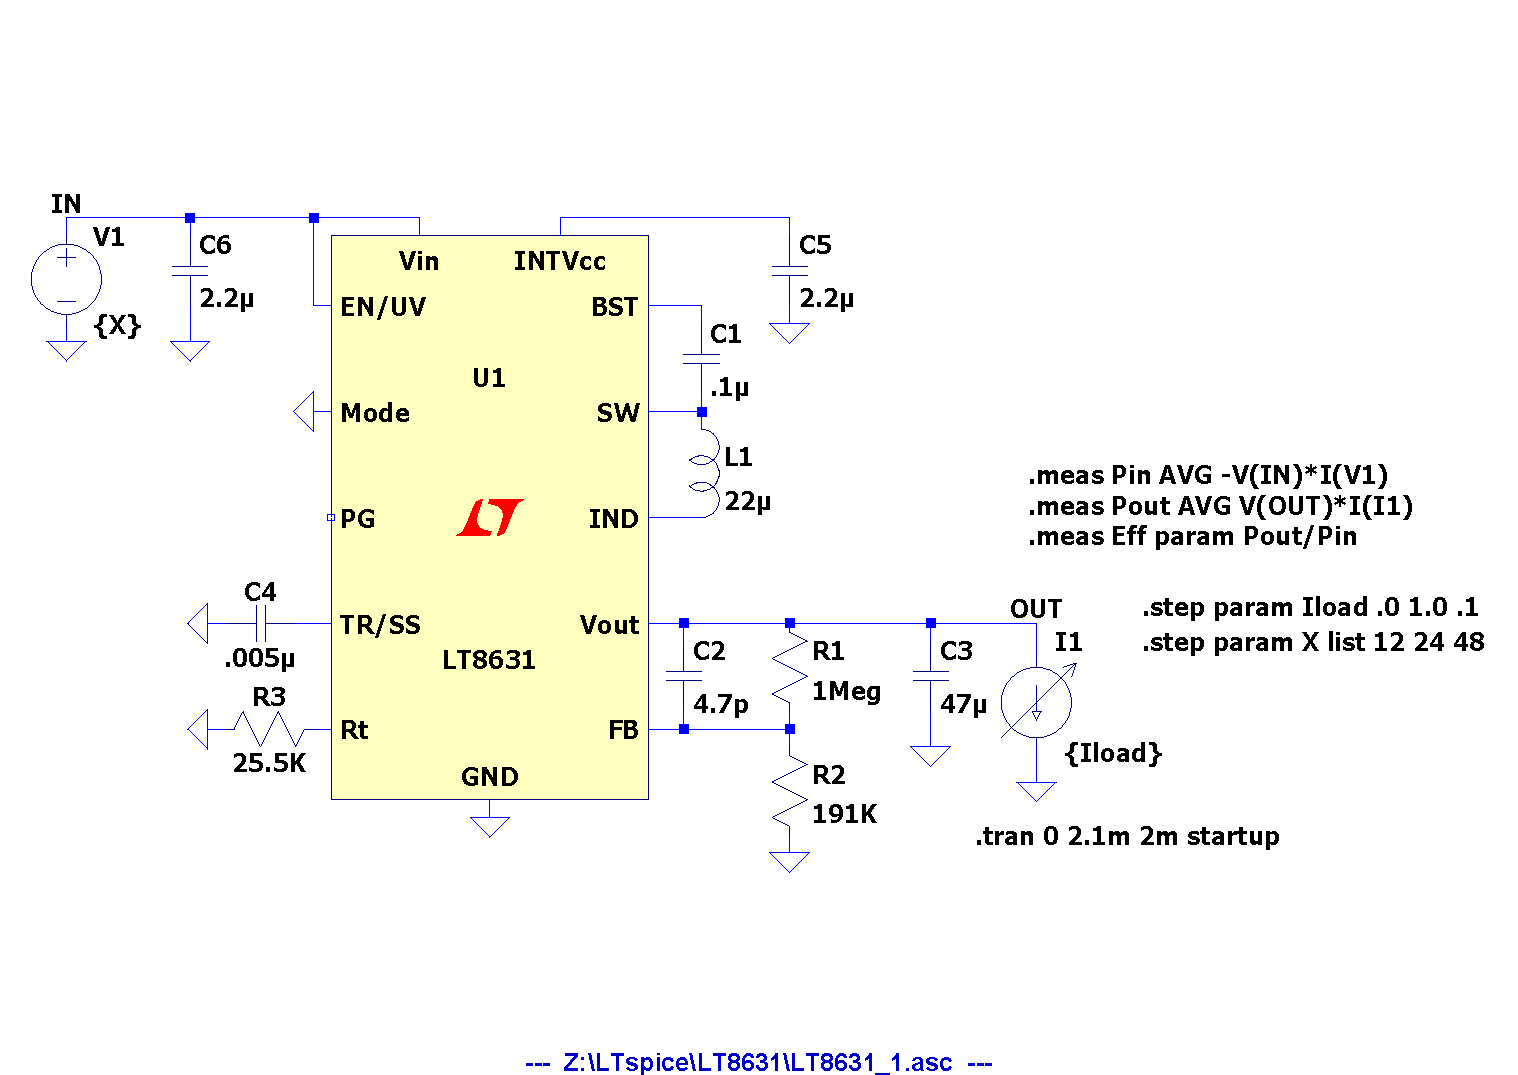
\includegraphics[page=1, width=0.6\textwidth]{figure/G01_asc.pdf}
    \caption{Efficiency at VOUT = 5V}
\end{figure}

\subsection{运行结果}

运行后,按 CTRL+L 打开 LTspice 的 log 文件,可以看到下面的输出,其中包含了 Eff 值。
选择 \textbf{Measurement: eff} ,右键,选择 \textbf{Plot .step'ed .meas data}。
在新打开的窗口中,CTRL+A 打开 \textbf{Add Traces},选择 \textbf{eff},可以得到下面的波形图。

\begin{figure}[!htb]
    \centering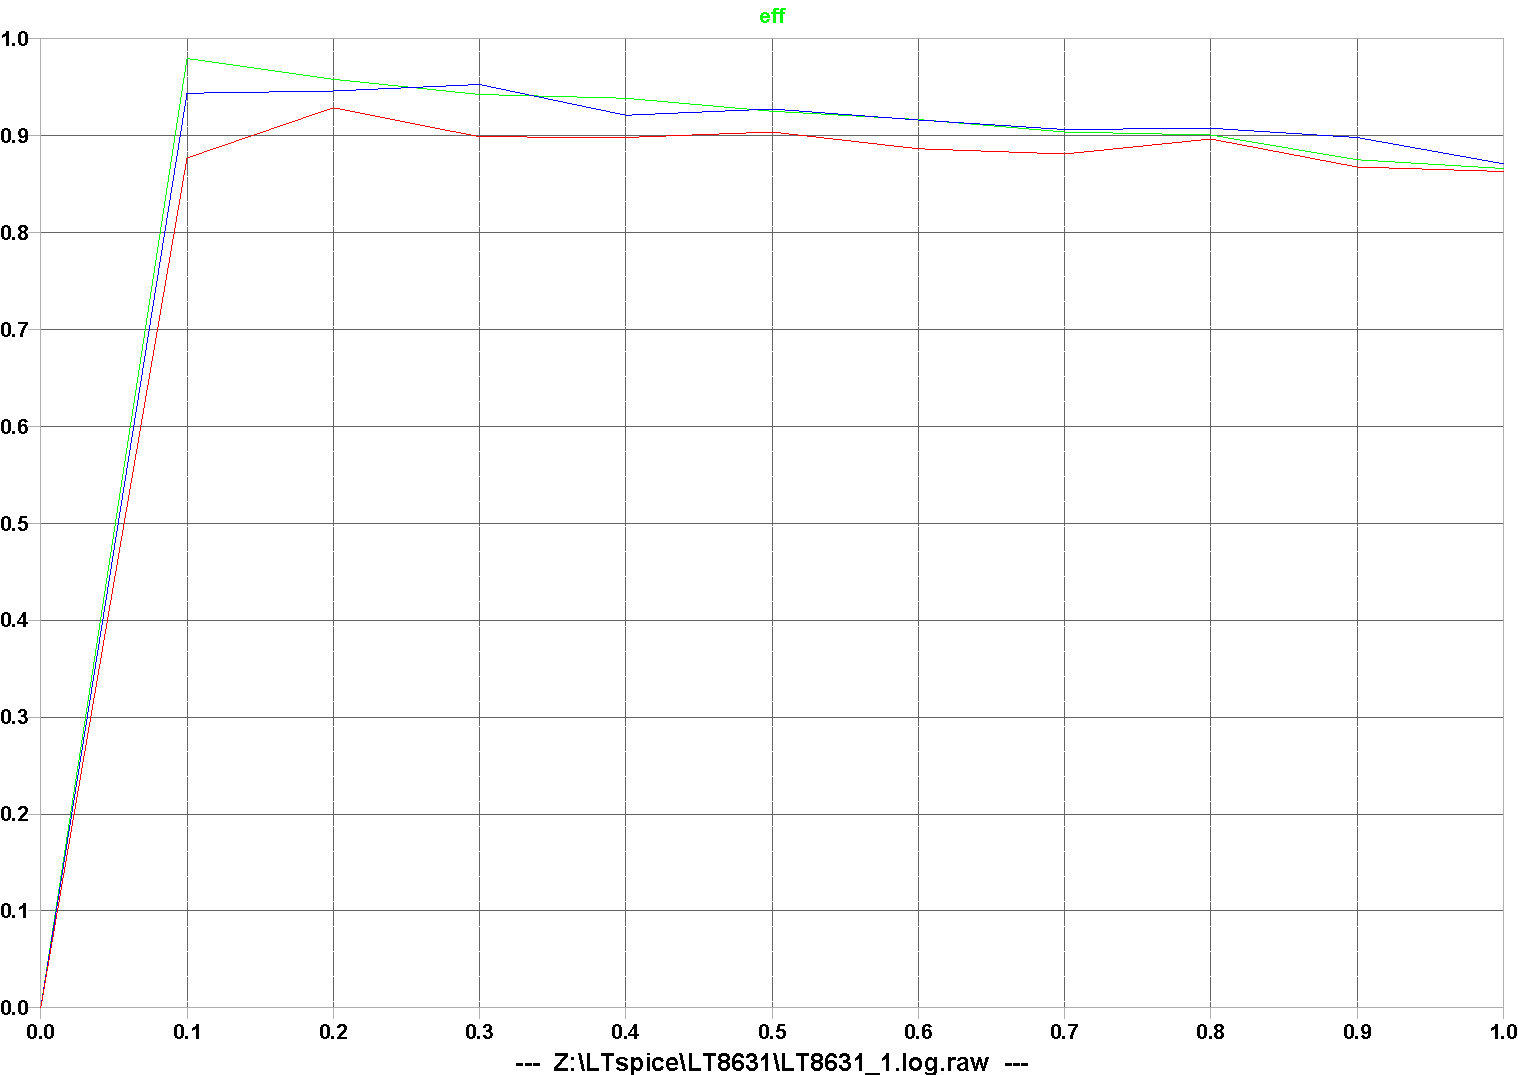
\includegraphics[page=1, width=0.6\textwidth]{figure/G01.pdf}
    \caption{Efficiency at VOUT = 5V}
\end{figure}

\section{Efficiency at VOUT = 3.3V}

\subsection{任务详细内容}

分别满足以下条件下,仿真实现datasheet中的图01中所示 Efficiency at VOUT = 3.3V。

$V_{IN} = 12V$

$V_{IN} = 24V$

$V_{IN} = 48V$

\subsection{功能描述}

通过阅读datasheet可知,修改 $V_{out}$ 为 3.3V ,需要将 R2 从 $191k\Omega$ 修改为 $324k\Omega$

\subsection{运行结果}

\begin{figure}[!htb]
    \centering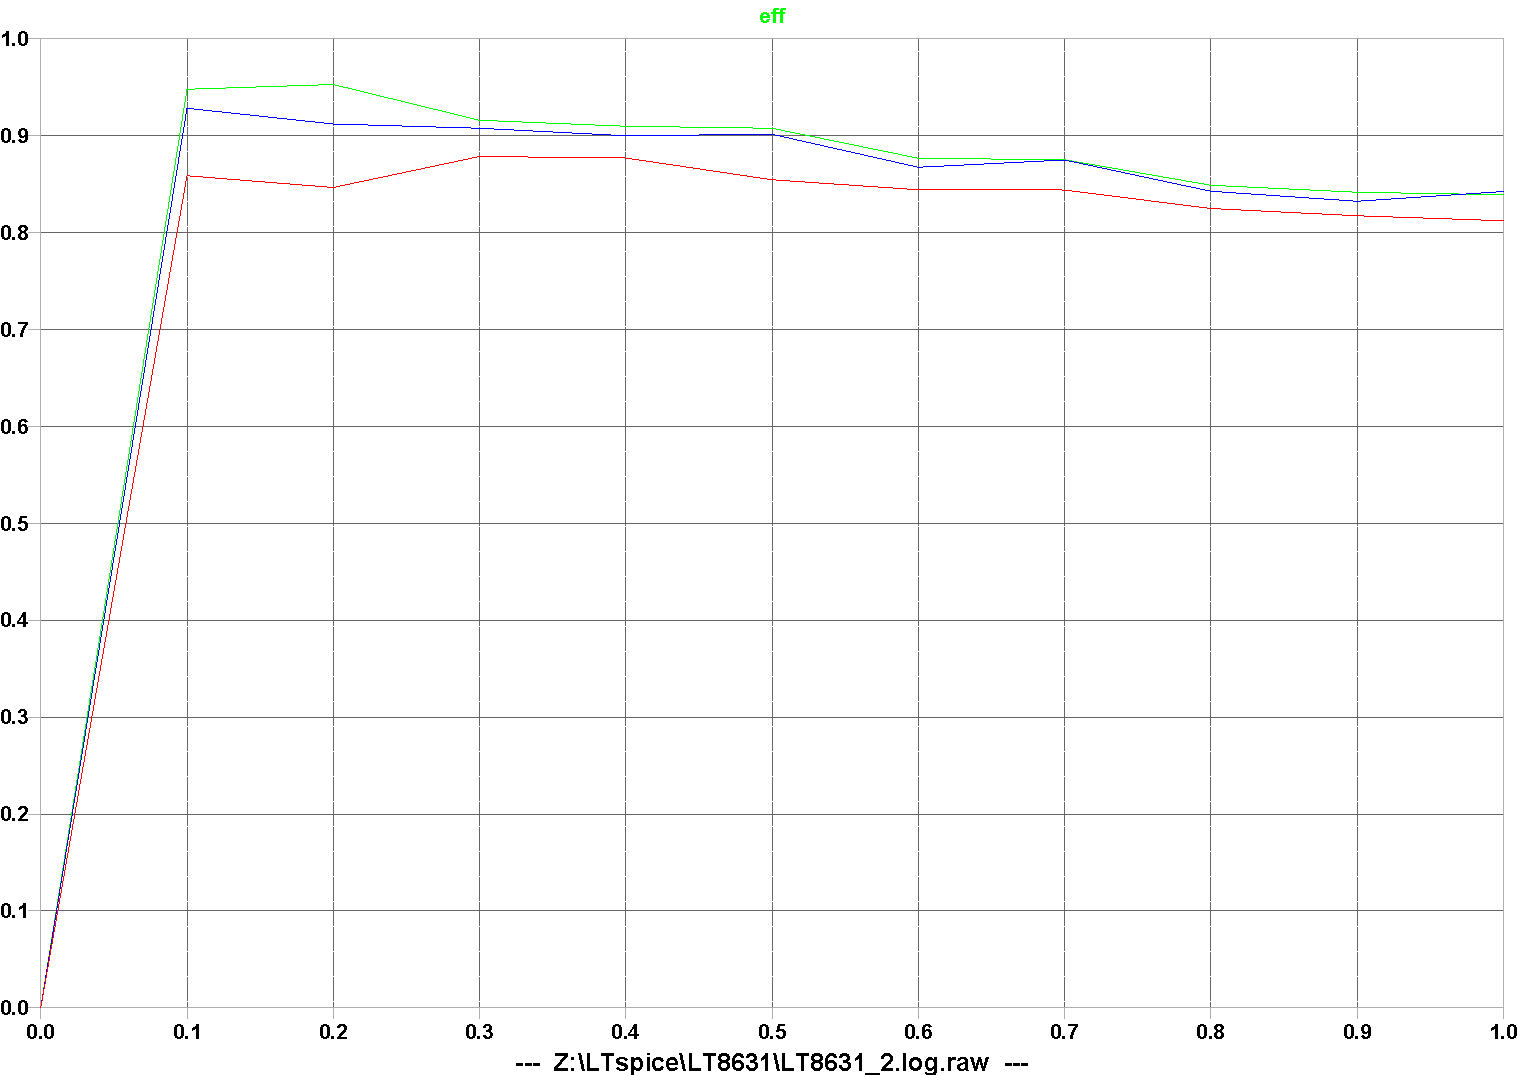
\includegraphics[page=1, width=0.6\textwidth]{figure/G02.pdf}
    \caption{Efficiency at VOUT = 3.3V}
\end{figure}

\section{Efficiency}

\subsection{任务详细内容}

满足以下条件下,SWITCHING FREQUENCY (kHz) 和 EFFICIENCY 的关系

$V_{IN} = 12V$

$V_{OUT} = 5V$

LOAD = 0.5A

$I_{LRIPPLE} = 0.4A$

\subsection{功能描述}

LT8631 的开关频率(Switching Frequency)是指内部同步开关的工作频率,可以通过 RT 引脚的外接电阻进行调节,范围为 100kHz 到 1MHz。开关频率会影响转换器的效率(Efficiency),即输出功率与输入功率的比值。一般来说,开关频率越高,效率越低,因为高频开关会导致更多的开关损耗和电磁干扰。开关频率越低,效率越高,但是需要更大的电感和电容来维持输出电压的稳定性。

LT8631 的数据手册给出了在不同输入电压、输出电压和负载电流的条件下,开关频率和效率的关系曲线。从曲线可以看出,开关频率和效率的关系并不是线性的,而是存在一个最佳的开关频率,使得效率达到最大值。这个最佳的开关频率取决于输入电压、输出电压和负载电流的大小,以及外部元件的选择。一般来说,当输入电压较高,输出电压较低,负载电流较大时,最佳的开关频率较低;反之,当输入电压较低,输出电压较高,负载电流较小时,最佳的开关频率较高。

如果要用数学公式来描述开关频率和效率的关系,可以使用下面的近似表达式:

$$\eta = \frac{V_{OUT}I_{OUT}}{V_{IN}I_{IN}} = \frac{V_{OUT}I_{OUT}}{V_{OUT}I_{OUT} + P_{SW} + P_{CON} + P_{Q}}$$

其中,$\eta$ 是效率,$V_{OUT}$ 是输出电压,$I_{OUT}$ 是负载电流,$V_{IN}$ 是输入电压,$I_{IN}$ 是输入电流,$P_{SW}$ 是开关损耗,$P_{CON}$ 是导通损耗,$P_{Q}$ 是静态损耗。开关损耗和开关频率成正比,导通损耗和负载电流的平方成正比,静态损耗和输入电压成正比。这个表达式可以用来估算不同开关频率下的效率,但是需要知道各种损耗的具体数值,这些数值可以从数据手册或者仿真软件中获取。

通过修改 $R_{RT}$ 的电阻值,可以控制 SWITCHING FREQUENCY (kHz)

\begin{table}[h]
    \centering
    \begin{tabular}{@{}rr@{}}
    \toprule
    Frequency (kHz) & $R_{RT} (k\Omega)$ \\ \midrule
    100             & 187                \\
    200             & 60.4               \\
    300             & 35.7               \\
    400             & 25.5               \\
    500             & 19.6               \\
    600             & 15.8               \\
    700             & 13.3               \\
    800             & 11.5               \\
    900             & 10                 \\
    1000            & 8.66               \\ \bottomrule
    \end{tabular}
    \caption{A table of frequency and resistance values}
    \label{tab:SW Frequency vs $R_T$ Value}
\end{table}

\begin{lstlisting}[language=Python, caption=G05]
    .step param Rt list 187k, 60.4k, 35.7k, 25.5k, 19.6k, 15.8k, 13.3k, 11.5k, 10k, 8.66k

    .tran 0 2.1m 2m startup
    
    .meas Pin AVG -V(IN)*I(V1)
    .meas Pout AVG V(OUT)*I(I1)
    .meas Eff param Pout/Pin
\end{lstlisting}

\subsection{运行结果}

遇到的问题: 横坐标是 $R_t$ 的值,而不是频率

\begin{figure}[!htb]
    \centering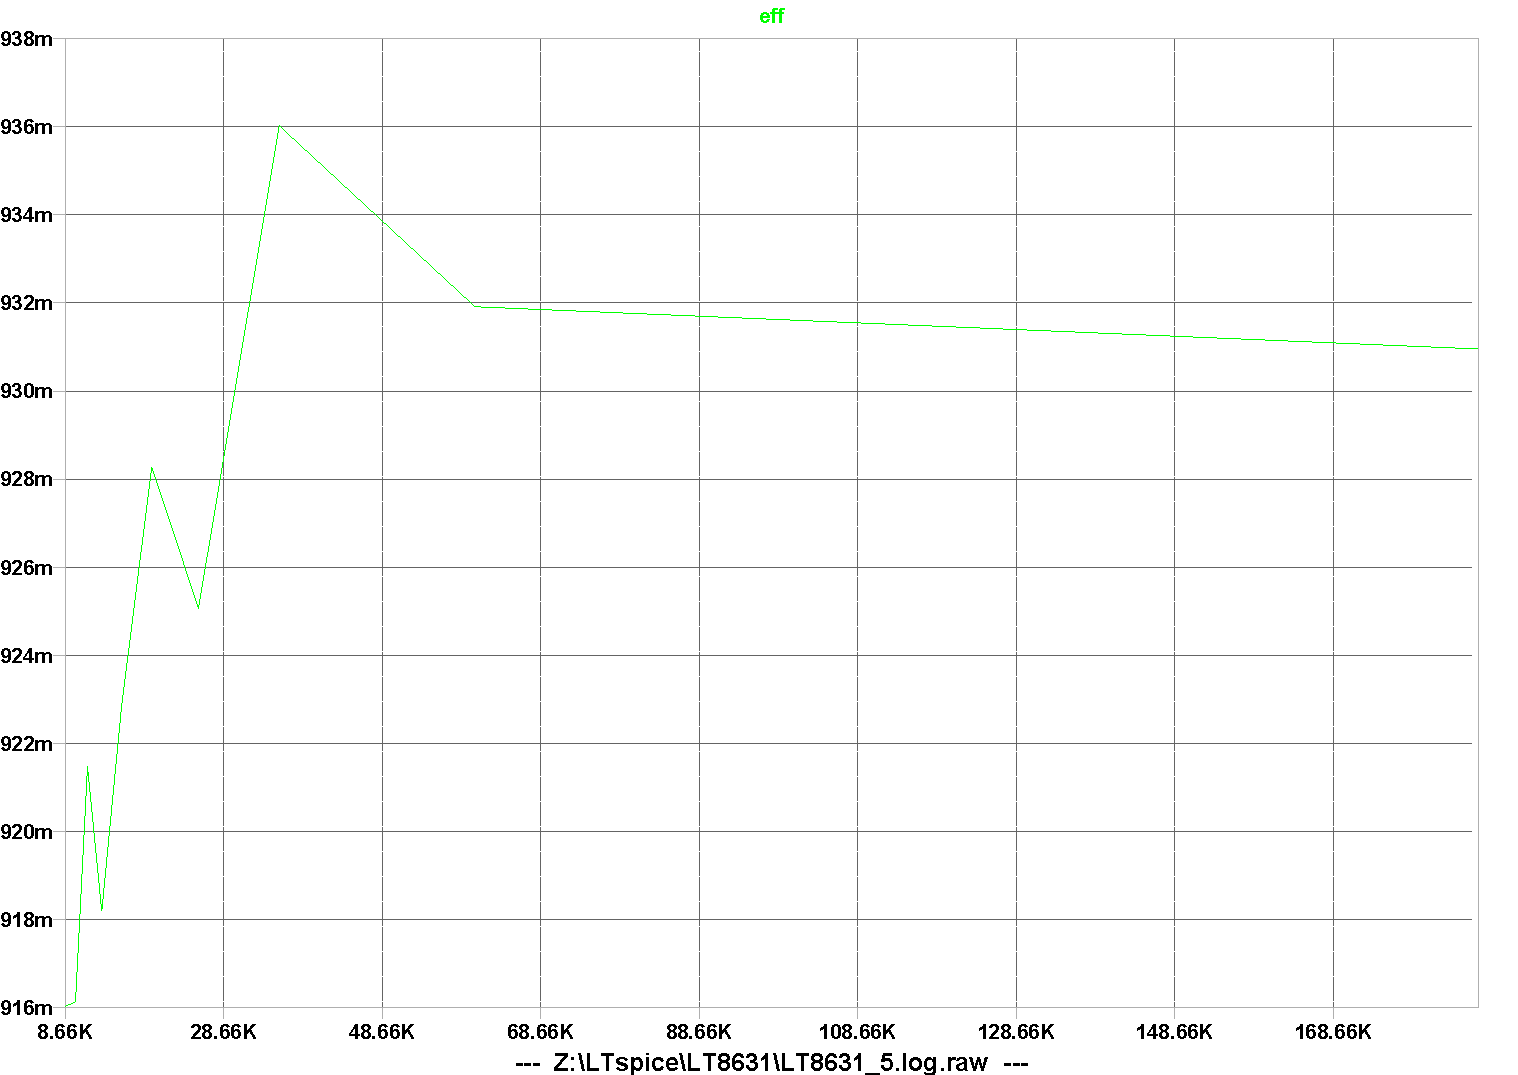
\includegraphics[page=1, width=0.6\textwidth]{figure/G05.pdf}
    \caption{Input Voltage Transient Response}
\end{figure}

\section{Burst Waveforms}

\subsection{任务详细内容}

满足以下条件下,仿真实现datasheet中的图26中所示 Burst Waveforms。

$V_{\text{IN}} = 12V$

LOAD = 5mA

\subsection{功能描述}

Burst Waveforms是一种输出波形,它包含一定数量的完整电平的波形周期,然后是一段较低电平的波形周期。
从完整电平到低电平的转换发生在波形的零交叉点。低电平可以设置在0到100\%之间的任意值。

$$
\text{Burst Waveforms} = \begin{cases}
V_{\text{max}} \sin(2\pi f t) & 0 \leq t \leq \frac{n}{f}\\
V_{\text{min}} \sin(2\pi f t) & \frac{n}{f} < t \leq \frac{m}{f}
\end{cases}
$$

其中,$V_{\text{max}}$是完整电平的电压,$V_{\text{min}}$是低电平的电压,$f$ 是波形的频率,$n$ 是完整电平的波形周期数,$m$ 是总的波形周期数。

为了测试 Burst Waveforms,先建立下面的电路图。

对比给出给出的演示电路,主要修改了以下几个参数:

\begin{itemize}
    \item V1 从 48 修改为 12
    \item Rload 从 5 修改为 \{5/0.005\}
\end{itemize}

\subsection{运行结果}

运行得到下面的波形图。

\begin{figure}[htbp]
    \centering\begin{minipage}[t]{0.48\textwidth}
        \centering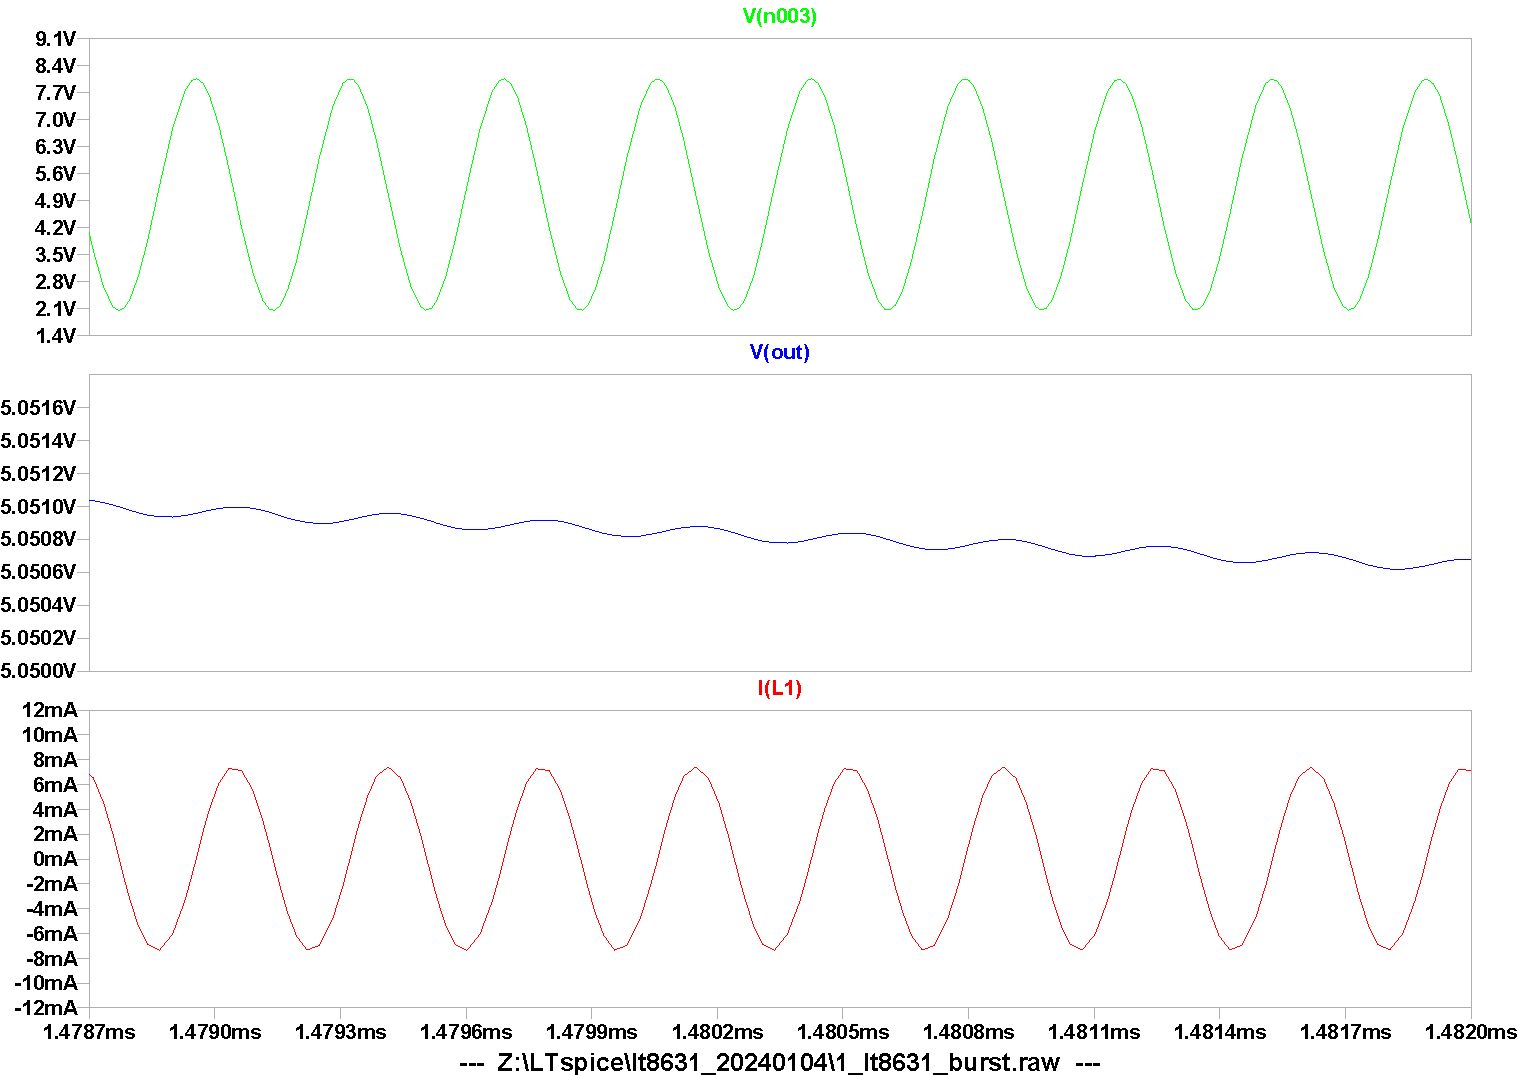
\includegraphics[page=1, width=0.9\textwidth]{figure/G26.pdf}
        \caption{Burst Waveforms}
    \end{minipage}
    \centering\begin{minipage}[t]{0.48\textwidth}
        \centering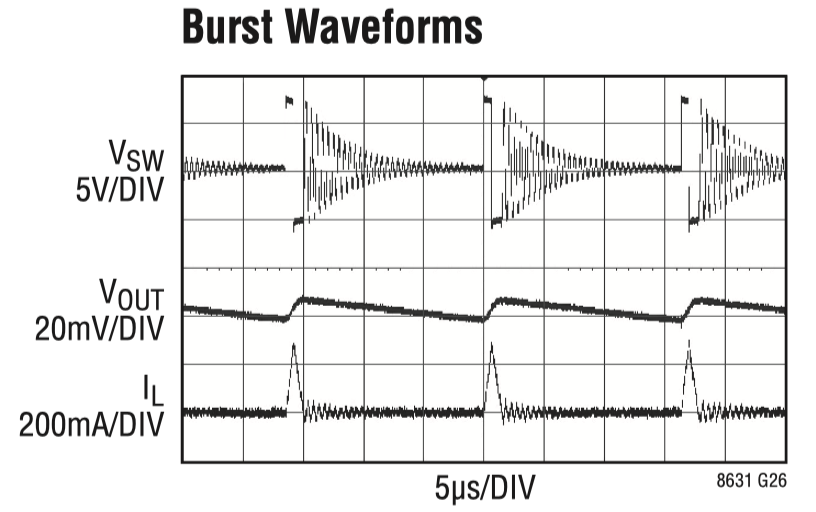
\includegraphics[width=0.9\linewidth]{figure/datasheet_G26.png}
        \caption{Burst Waveforms}
    \end{minipage}
\end{figure}

\section{Burst Waveforms 2}

\subsection{任务详细内容}

满足以下条件下,仿真实现datasheet中的图27中所示 Burst Waveforms。

$V_{\text{IN}} = 100V$

LOAD = 50mA

\subsection{功能描述}

Burst Waveforms是一种输出波形,它包含一定数量的完整电平的波形周期,然后是一段较低电平的波形周期。
从完整电平到低电平的转换发生在波形的零交叉点。低电平可以设置在0到100\%之间的任意值。

$$
\text{Burst Waveforms} = \begin{cases}
V_{\text{max}} \sin(2\pi f t) & 0 \leq t \leq \frac{n}{f}\\
V_{\text{min}} \sin(2\pi f t) & \frac{n}{f} < t \leq \frac{m}{f}
\end{cases}
$$

其中,$V_{\text{max}}$是完整电平的电压,$V_{\text{min}}$是低电平的电压,$f$ 是波形的频率,$n$ 是完整电平的波形周期数,$m$ 是总的波形周期数。

为了测试 Burst Waveforms,先建立下面的电路图。

对比给出给出的演示电路,主要修改了以下几个参数:

\begin{itemize}
    \item V1 从 48 修改为 100
    \item Rload 从 5 修改为 \{5/0.05\}
\end{itemize}

\begin{figure}[!htb]
    \centering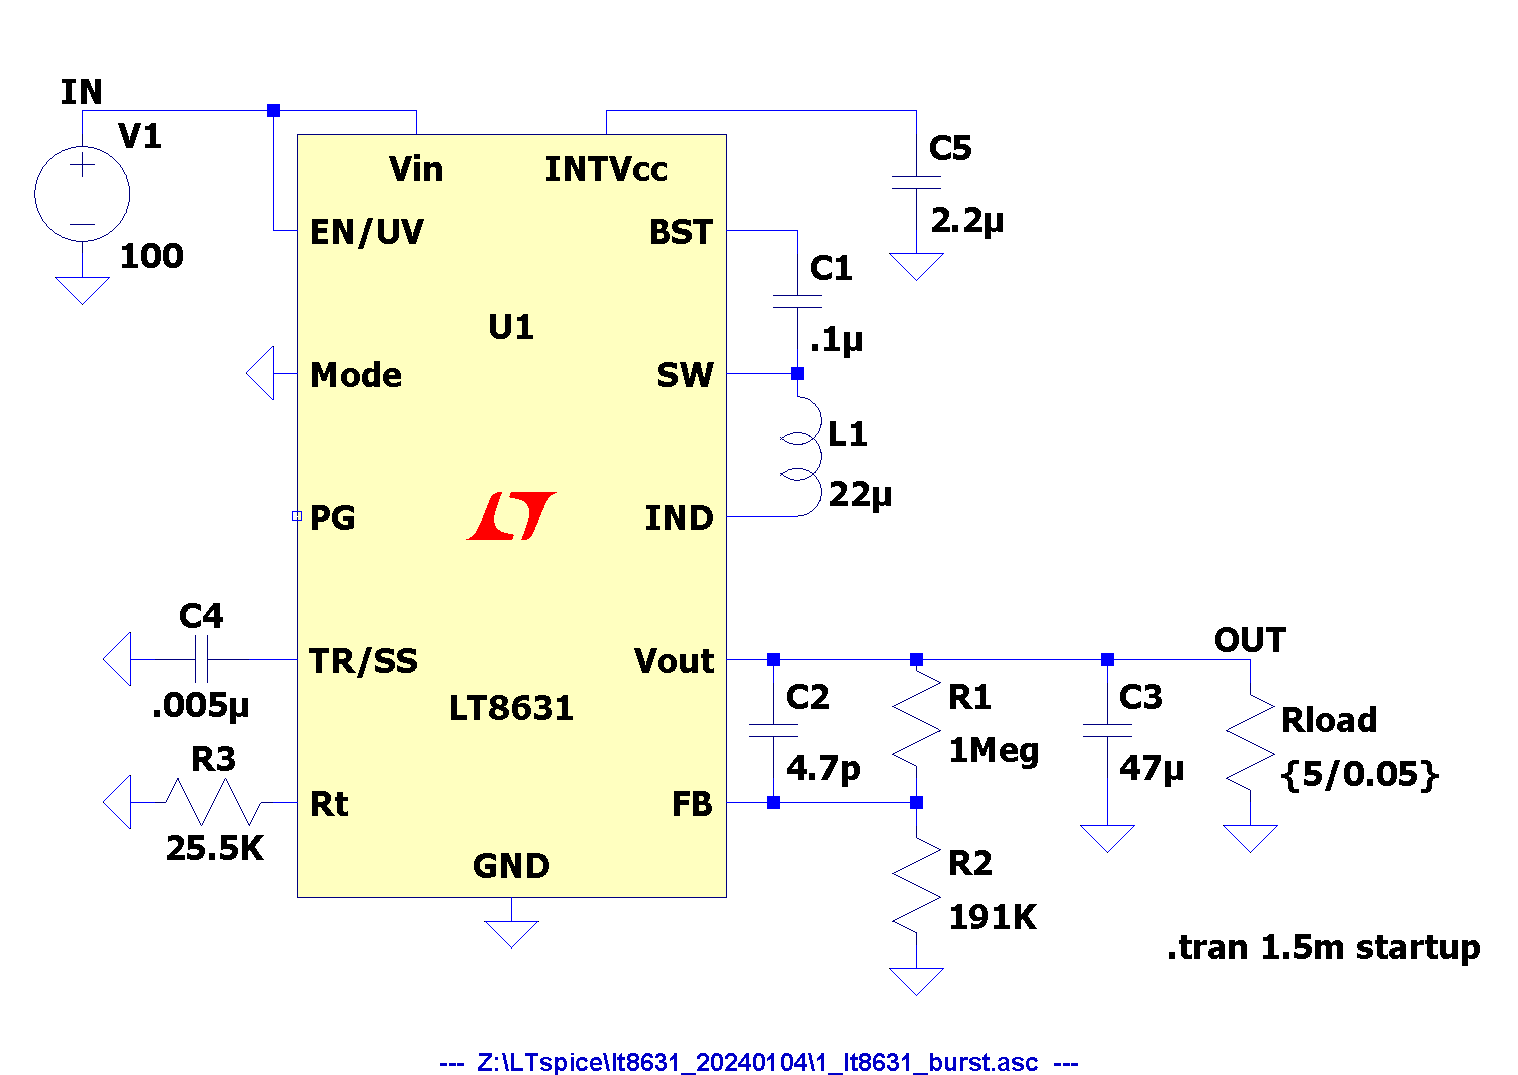
\includegraphics[page=1, width=0.6\textwidth]{figure/1_lt8631_burst_asc.pdf}
    \caption{Burst Waveforms 2}
\end{figure}

\subsection{运行结果}

运行得到下面的波形图。

\begin{figure}[htbp]
    \centering\begin{minipage}[t]{0.48\textwidth}
        \centering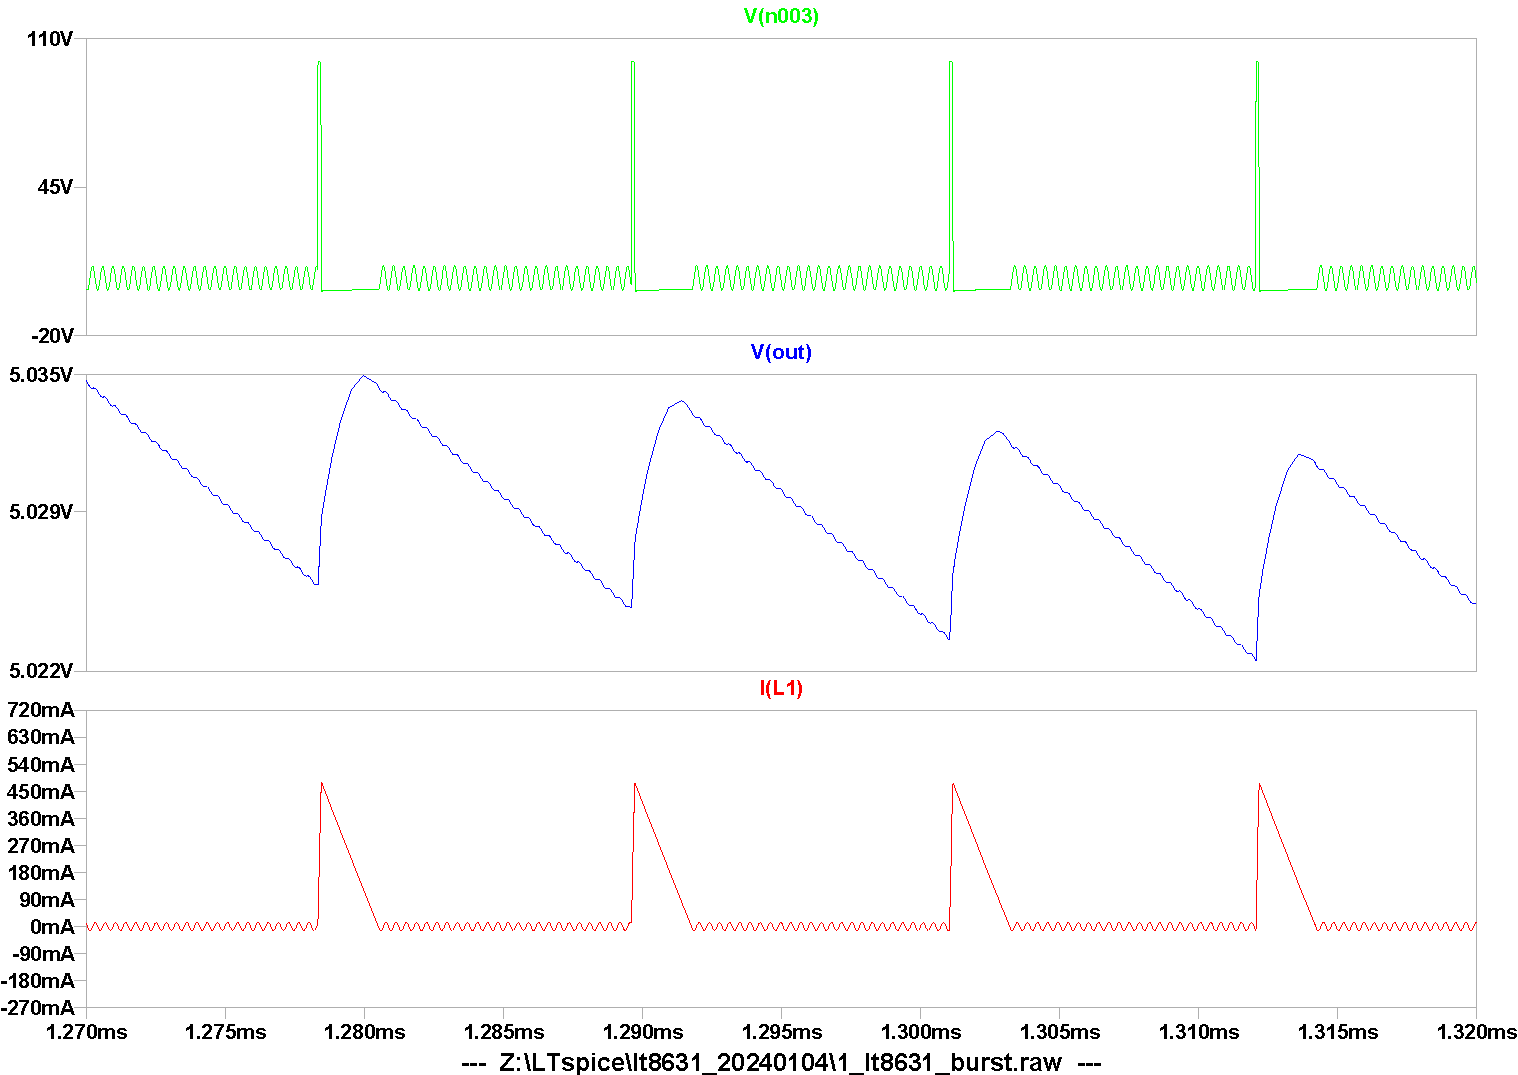
\includegraphics[page=1, width=0.9\textwidth]{figure/1_lt8631_burst_2.pdf}
        \caption{Burst Waveforms 2}
    \end{minipage}
    \centering\begin{minipage}[t]{0.48\textwidth}
        \centering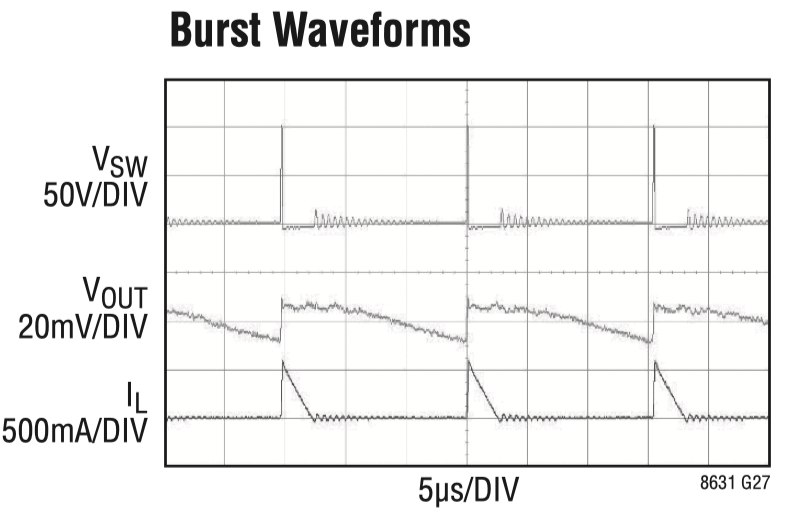
\includegraphics[width=0.9\linewidth]{figure/datasheet_G27.png}
        \caption{Burst Waveforms 2}
    \end{minipage}
\end{figure}

\section{Switching Waveforms}

\subsection{任务详细内容}

满足以下条件下,仿真实现datasheet中的图28中所示 Switching Waveforms。

$V_{\text{IN}} = 12V$

LOAD = 5mA

\subsection{功能描述}

Switching Waveforms的含义是指在电力电子转换器中,开关元件的电压和电流随时间变化的波形。
这些波形反映了开关元件的工作状态,转换器的输出特性,以及电磁干扰(EMI)的产生。
通过调整开关波形的形状,可以优化转换器的效率,稳定性,和EMI控制。开关波形的分析和合成是电力电子技术的重要内容。

电磁干扰(EMI)是一种不希望存在的信号,它对电子设备或系统的正常工作会造成有害影响。

为了测试 Switching Waveforms,先建立下面的电路图。

\begin{figure}[!htb]
    \centering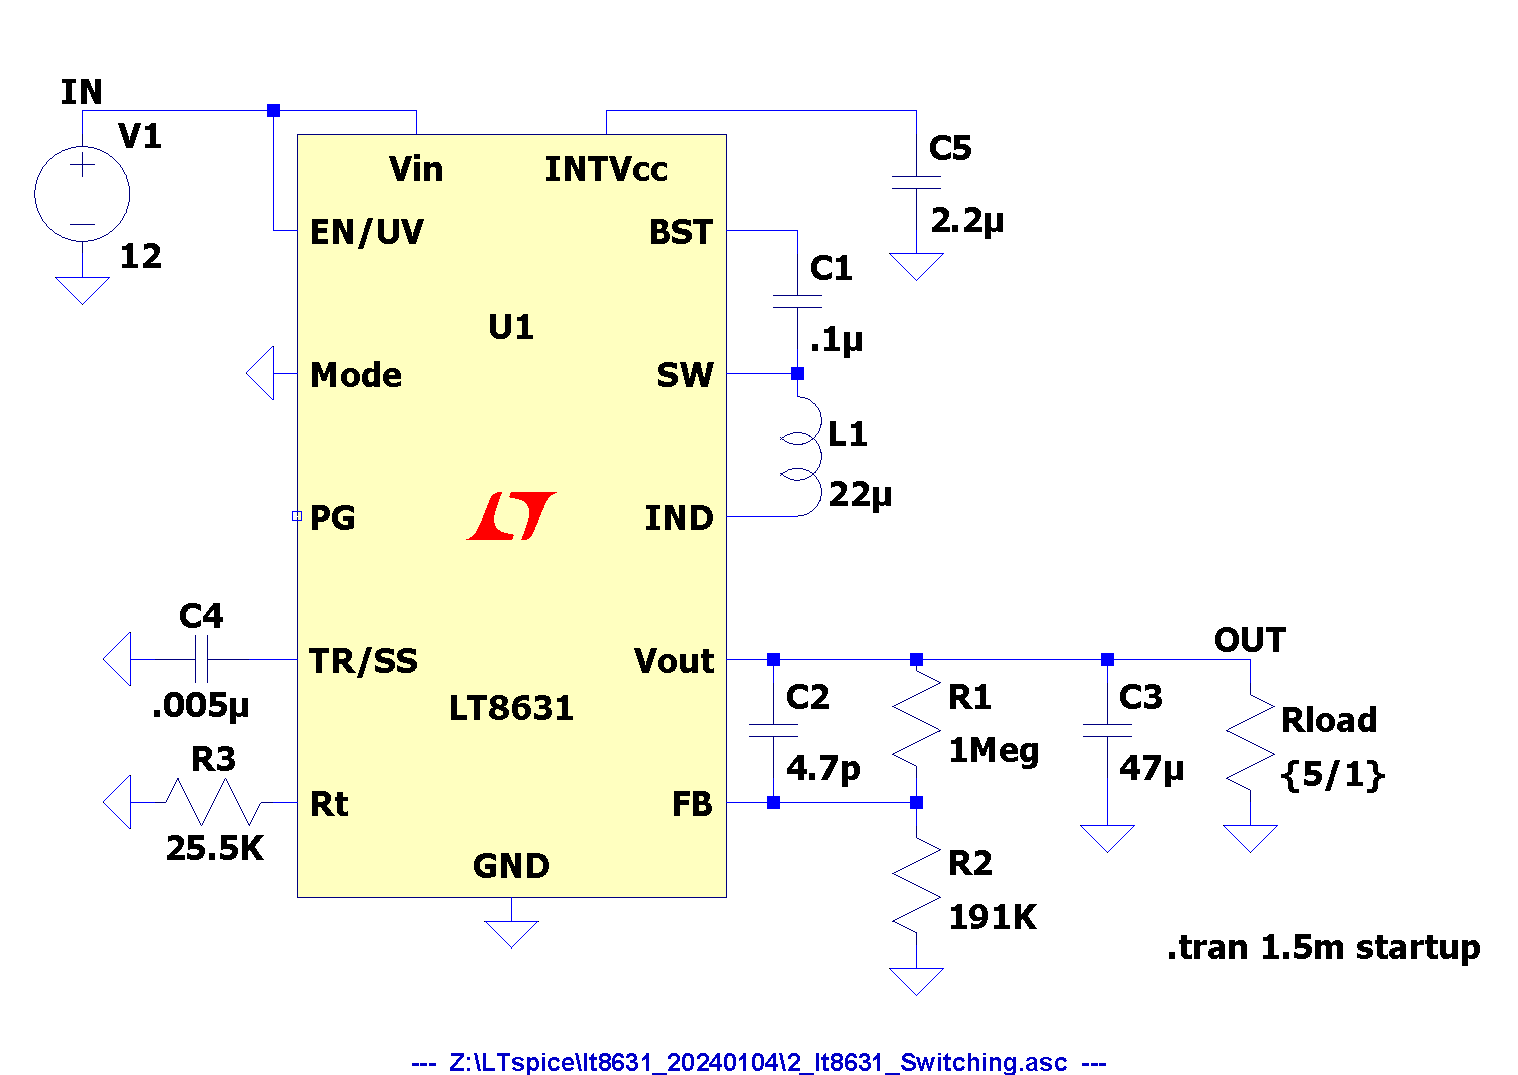
\includegraphics[page=1, width=0.6\textwidth]{figure/2_lt8631_Switching_asc.pdf}
    \caption{Switching Waveforms}
\end{figure}

\subsection{运行结果}

运行得到下面的波形图。

\begin{figure}[htbp]
    \centering\begin{minipage}[t]{0.48\textwidth}
        \centering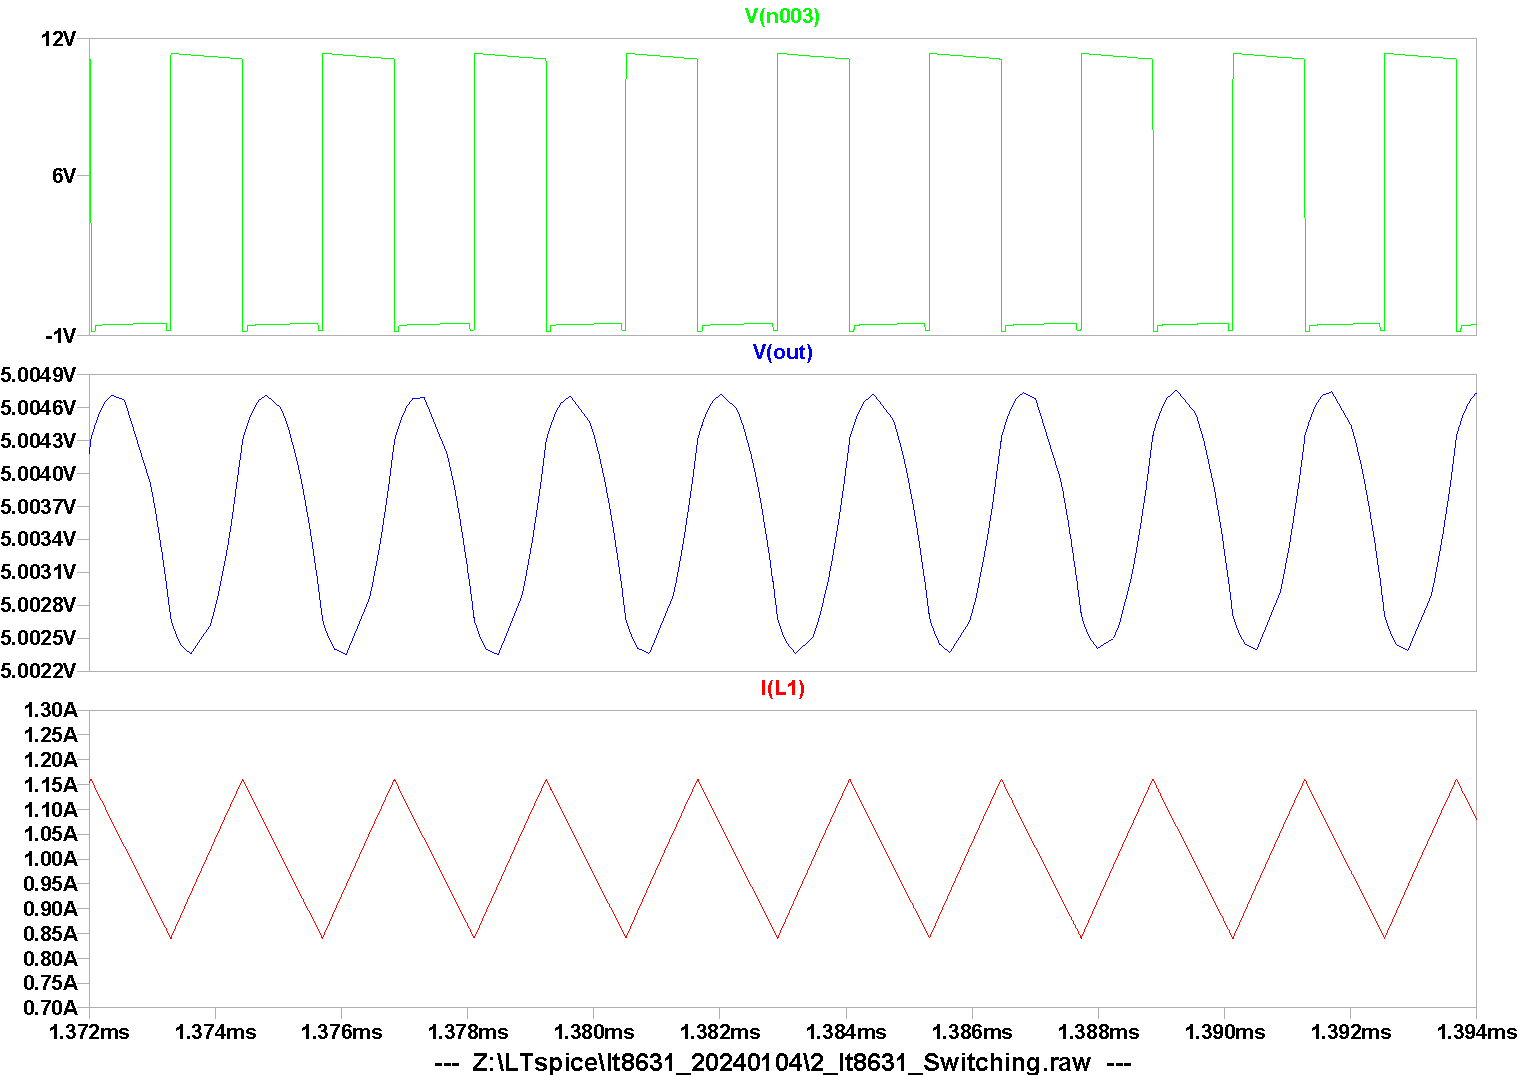
\includegraphics[page=1, width=0.9\textwidth]{figure/2_lt8631_Switching_2.pdf}
        \caption{Switching Waveforms}
    \end{minipage}
    \centering\begin{minipage}[t]{0.48\textwidth}
        \centering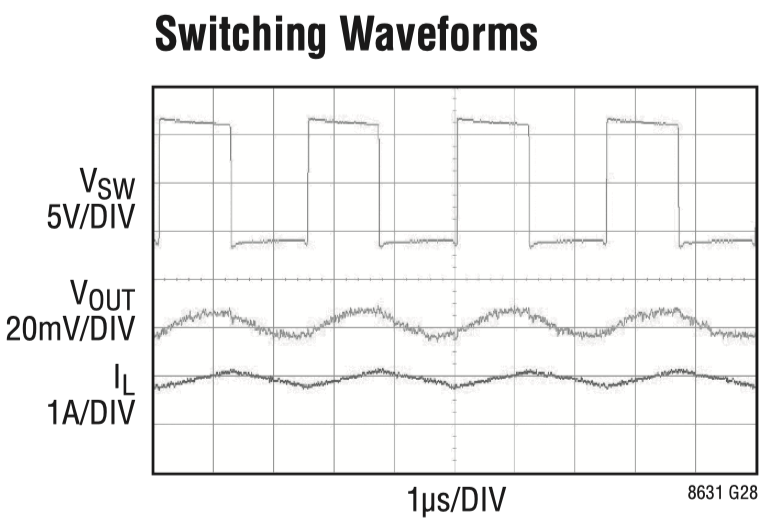
\includegraphics[width=0.9\linewidth]{figure/datasheet_G28.png}
        \caption{Switching Waveforms}
    \end{minipage}
\end{figure}

\section{Switching Waveforms 2}

\subsection{任务详细内容}

满足以下条件下,仿真实现datasheet中的图29中所示 Switching Waveforms。

$V_{\text{IN}} = 12V$

LOAD = 5mA

\subsection{功能描述}

为了测试 Switching Waveforms,电路图基本同上,需要修改的是 $V_{\text{IN}} = 100V$。

\subsection{运行结果}

运行得到下面的波形图。

\begin{figure}[htbp]
    \centering\begin{minipage}[t]{0.48\textwidth}
        \centering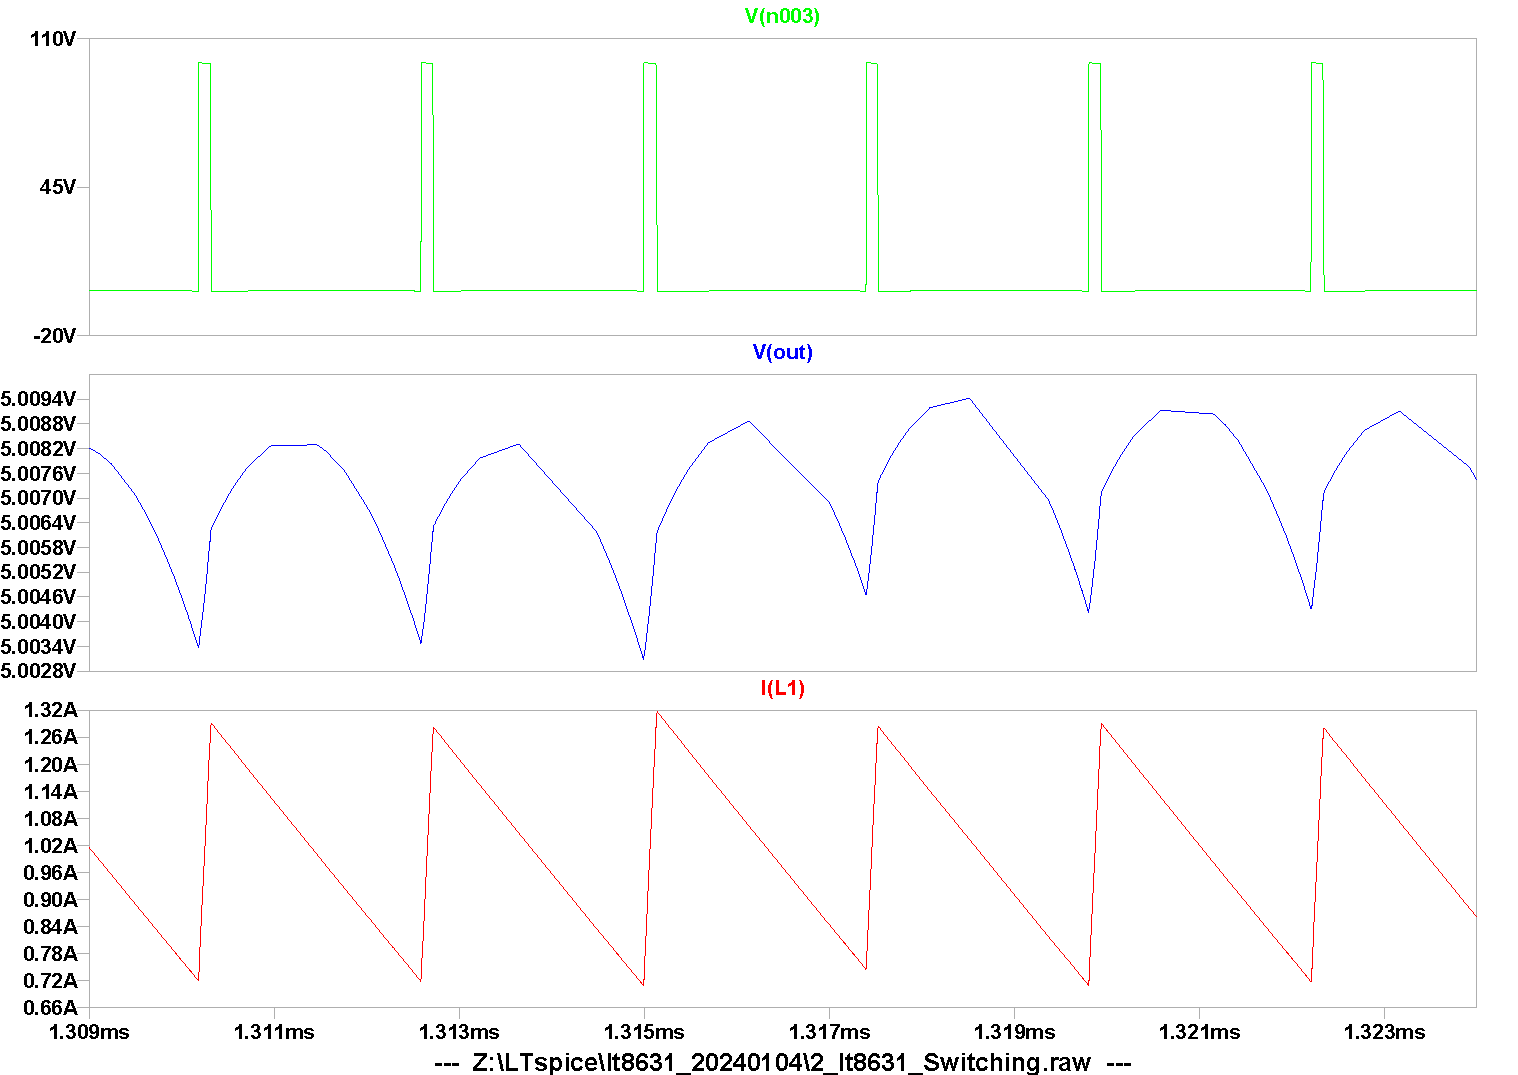
\includegraphics[page=1, width=0.9\textwidth]{figure/G29.pdf}
        \caption{Switching Waveforms}
    \end{minipage}
    \centering\begin{minipage}[t]{0.48\textwidth}
        \centering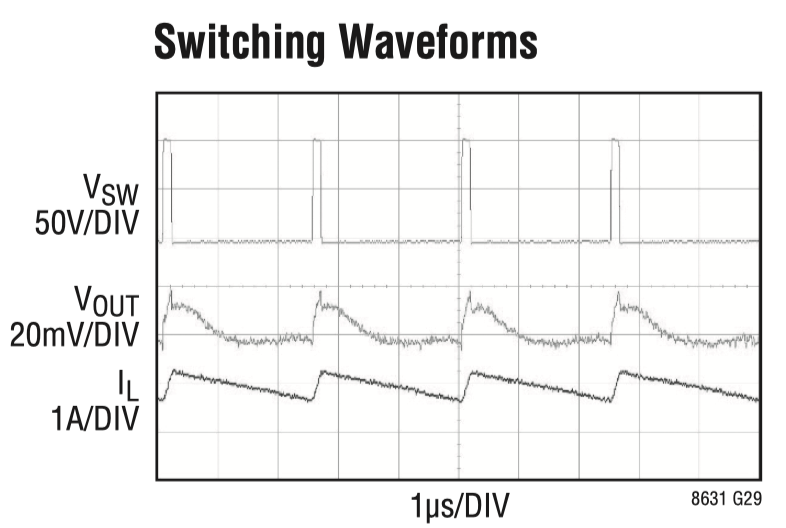
\includegraphics[width=0.9\linewidth]{figure/datasheet_G29.png}
        \caption{Switching Waveforms}
    \end{minipage}
\end{figure}

\section{Load Transient Response}

\subsection{任务详细内容}

满足以下条件下,仿真实现datasheet中的图30中所示 Load Transient Response。

200mA to 800mA LOAD TRANSIENT

$V_{\text{IN}} = 15V$

\subsection{功能描述}

Load Transient Response(负载瞬态响应)是指电路在负载电流发生快速变化时,输出电压的变化情况。
理想情况下,输出电压应该保持恒定,不受负载变化的影响。
但实际上,输出电压会出现一定的波动,如果超过了允许的电压容差范围,就会影响电路的正常工作。

负载瞬态响应的主要影响因素有以下几个:

\begin{itemize}
    \item 电路的频率响应,包括交越频率和稳定性。交越频率影响了电路的调节时间,即从负载变化开始到输出电压恢复到稳态值的时间。交越频率越高,调节时间越短。
    \item 输出电容的大小、类型和位置。输出电容相当于一个能量储存器,可以缓冲负载变化引起的电压波动。输出电容越大,电压波动越小。输出电容的寄生效应,如电感和电阻,也会影响负载瞬态响应。
    \item 负载电流的变化幅度和速率。负载电流变化越大,电压波动越大。负载电流变化越快,电压波动越剧烈。
\end{itemize}

负载瞬态响应是评价电压调节器性能的一个重要指标,尤其是对于数字电路等对电压敏感的应用。为了减小负载瞬态响应的影响,通常需要选择合适的电压调节器和输出电容,并进行测试和验证。

为了测试 Load Transient Response,先建立下面的电路图。

对比给出给出的演示电路,主要修改了以下几个参数:

\begin{itemize}
    \item V1 从 48 修改为 15
    \item Rload 从 5 修改为 \{5/0.2\}
    \item 添加 V2 为 \textbf{PULSE(0 10 0 1u 1u 150u 300u)}。这是为了模拟一个脉冲信号,用于控制开关管 M1 的导通和截止。这样可以在输出端产生一个周期性的负载瞬态,从而观察 LT8631 的瞬态响应。
    \item 添加 Rload1 为 \{5/0.6\}。这是为了增加一个并联的负载电阻,用于在 M1 导通时提供额外的负载电流。这样可以测试 LT8631 在重负载条件下的效率和输出纹波。 
    \item 添加 M1 为 BSB012NE2LX。这是为了选择一个合适的开关管,用于在 V2 的控制下切换负载电流。BSB012NE2LX 是一种 N 沟道 MOSFET,具有低导通电阻和低栅极电荷,适用于高频开关应用。
\end{itemize}

\begin{figure}[!htb]
    \centering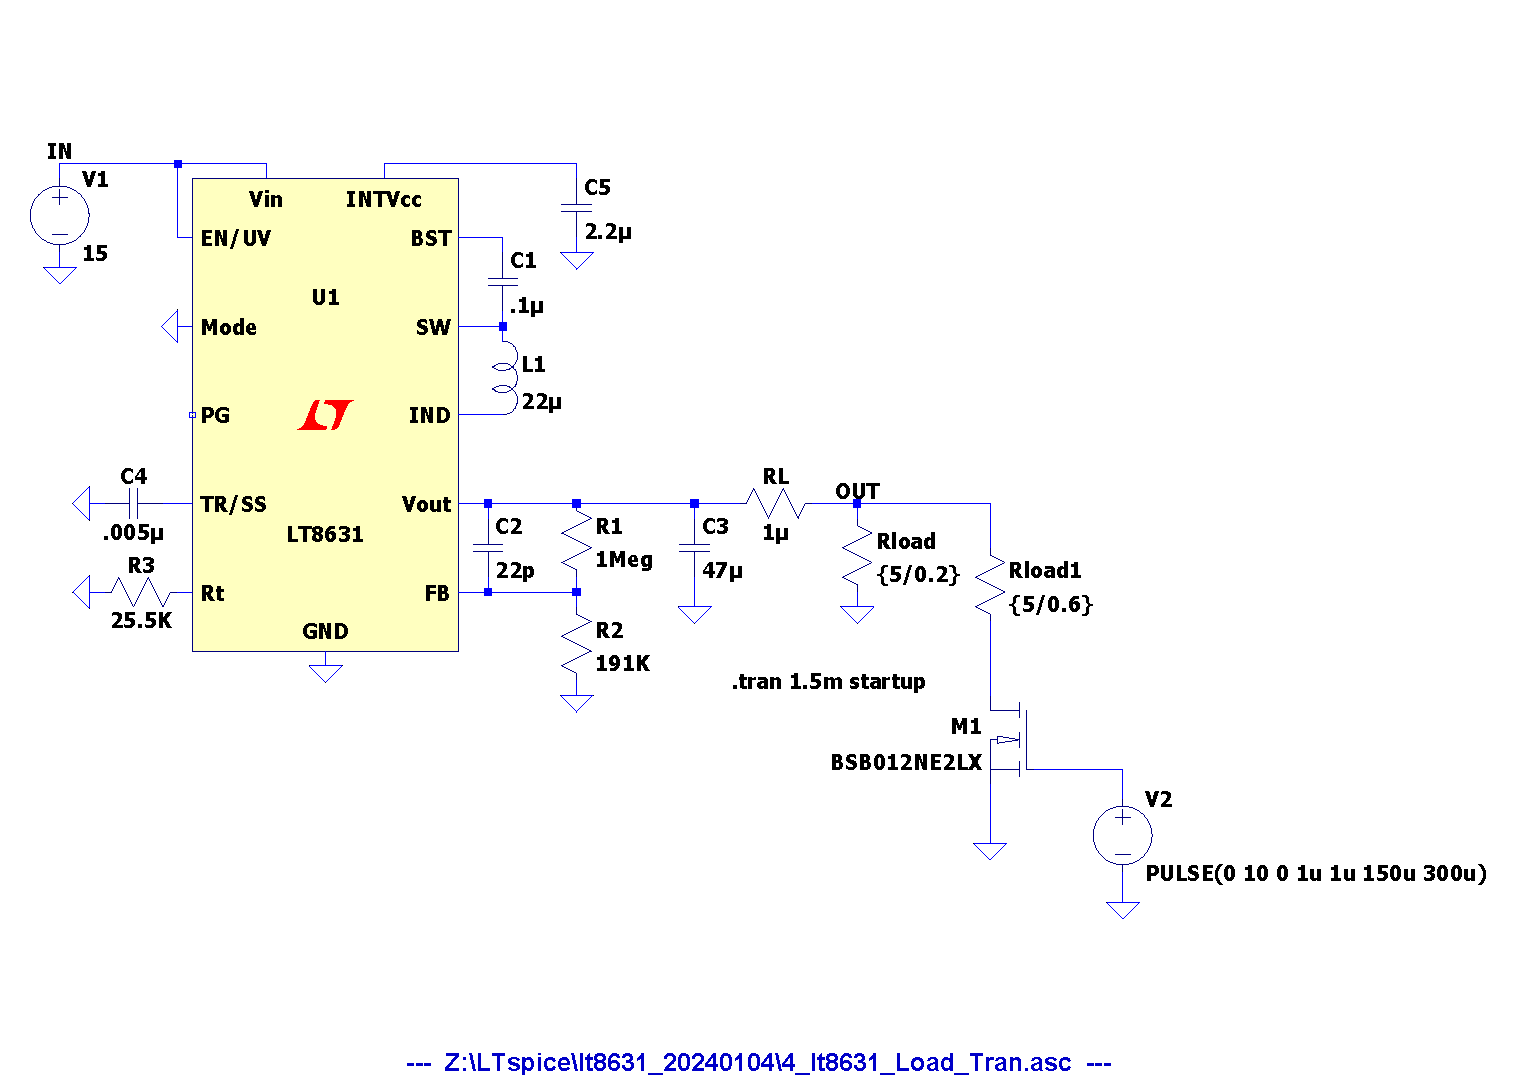
\includegraphics[page=1, width=0.6\textwidth]{figure/4_lt8631_Load_Tran_asc.pdf}
    \caption{Load Transient Response}
\end{figure}

\subsection{运行结果}

运行得到下面的波形图。

\begin{figure}[htbp]
    \centering\begin{minipage}[t]{0.48\textwidth}
        \centering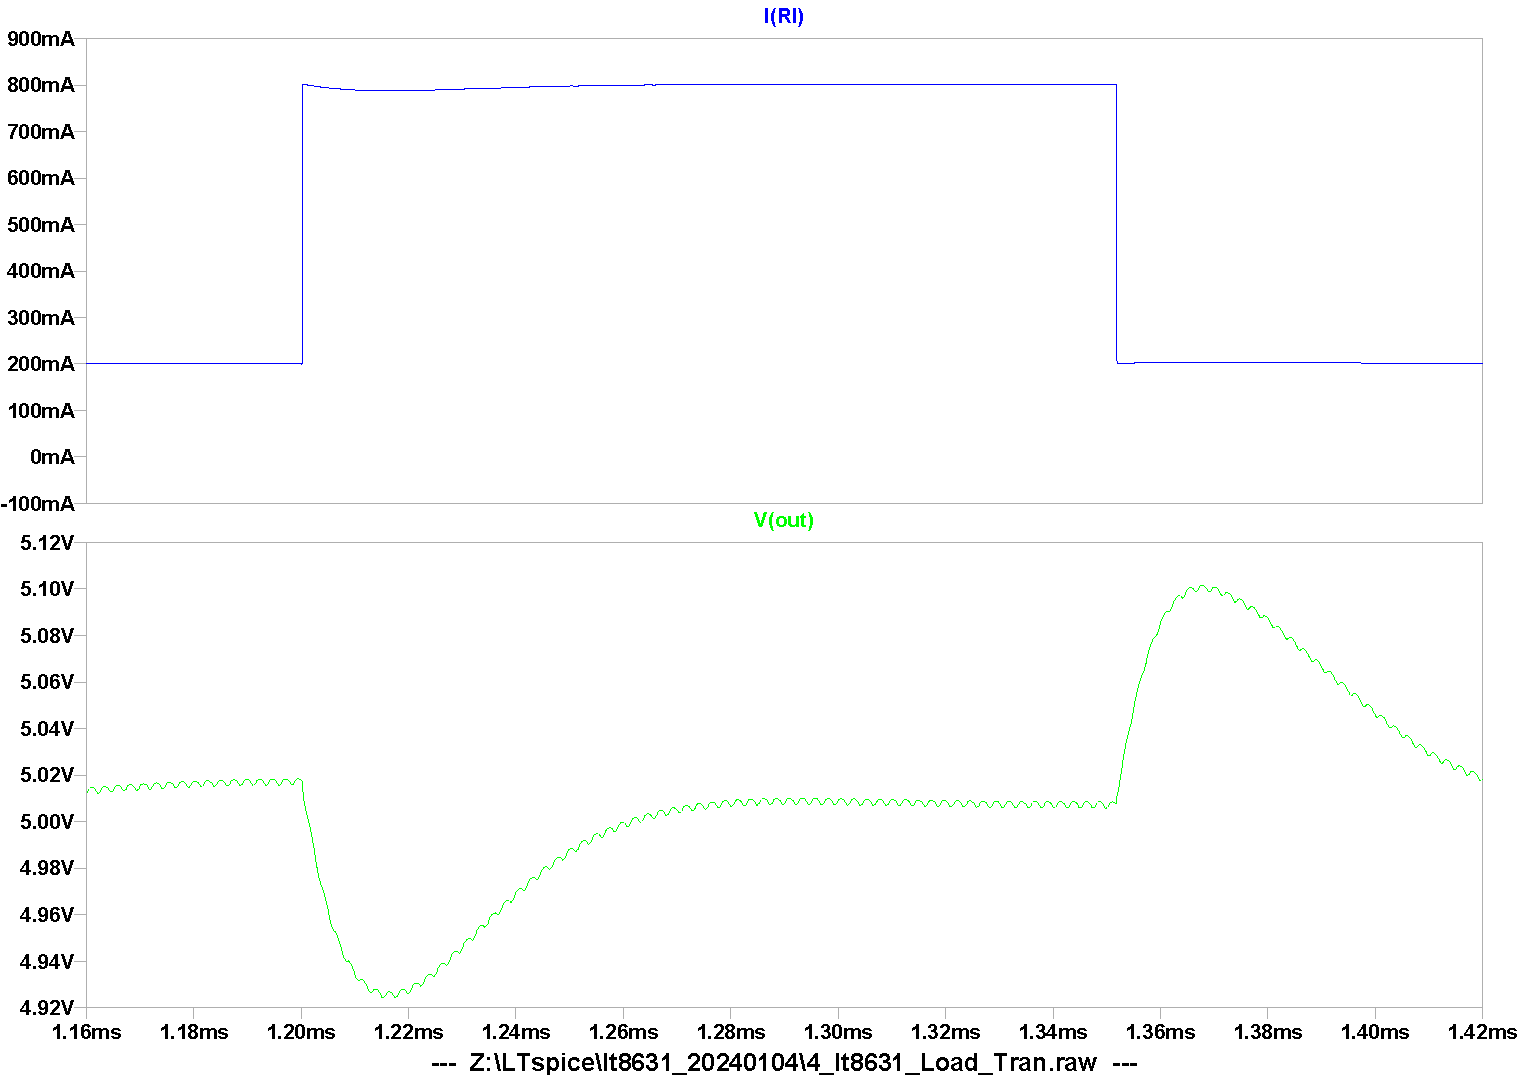
\includegraphics[page=1, width=0.9\textwidth]{figure/4_lt8631_Load_Tran_2.pdf}
        \caption{Load Transient Response}
    \end{minipage}
    \centering\begin{minipage}[t]{0.48\textwidth}
        \centering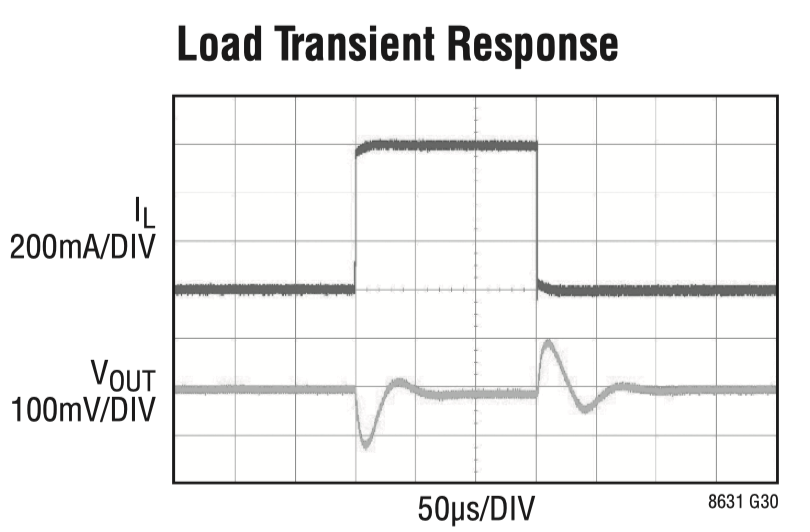
\includegraphics[width=0.9\linewidth]{figure/datasheet_G30.png}
        \caption{Load Transient Response}
    \end{minipage}
\end{figure}

\section{Input Voltage Transient Response}

\subsection{任务详细内容}

满足以下条件下,仿真实现datasheet中的图31中所示 Input Voltage Transient Response。

12V to 100V INPUT VOLTAGE TRANSIENT

LOAD = 100mA

$C_{\text{OUT}} = 2 \times 47µF$

\subsection{功能描述}

% 请解释Input Voltage Transient Response的含义。
% 请描述LT8631的datasheet中的Input Voltage Transient Response的含义。

Input Voltage Transient Response是指电路系统在输入电压发生突变时的输出电压变化情况。
一般来说,电路系统的输入电压会受到外界因素的影响,例如雷击、设备故障、电容器开关等,导致输入电压出现瞬态过电压。
这些瞬态过电压可能会对电路系统造成损坏或性能下降,因此需要设计合适的电路来应对输入电压的瞬态变化,并使输出电压尽快恢复到稳态值。

电路系统的瞬态响应可以用以下几个参数来描述:

\begin{itemize}
    \item 上升时间:指输出电压从一个低值变化到一个高值所需的时间,通常取10\%和90\%作为低值和高值。
    \item 过冲量:指输出电压超过稳态值的幅度。
    \item 调节时间:指输出电压从瞬态变化到稳态所需的时间,通常定义为输出电压进入并保持在一个误差范围内的时间。
    \item 延迟时间:指输出电压达到稳态值一半所需的时间。
    \item 峰值时间:指输出电压达到第一个过冲峰值所需的时间。
    \item 稳态误差:指输出电压达到稳态后与期望值的差值。
\end{itemize}

电路系统的瞬态响应还可以根据阻尼情况分为以下三种类型:

\begin{itemize}
    \item 欠阻尼:指输出电压在一个衰减的包络内振荡,阻尼越小,振荡越多,达到稳态越慢。
    \item 临界阻尼:指输出电压在不振荡的情况下最快达到稳态值。
    \item 过阻尼:指输出电压在不振荡的情况下达到稳态值比临界阻尼慢。
\end{itemize}

为了测试Input Voltage Transient Response,先建立下面的电路图。

对比给出给出的演示电路,主要修改了以下几个参数:

\begin{itemize}
    \item V1 从 48 修改为 15
    \item 添加 C6 为 \{47µ\}。这是为了增加一个输入电容,用于滤除输入电压的噪声和纹波。这样可以提高 LT8631 的抗干扰能力和输出质量。
    \item Rload 从 5 修改为 \{5/0.1\}
\end{itemize}

\begin{figure}[!htb]
    \centering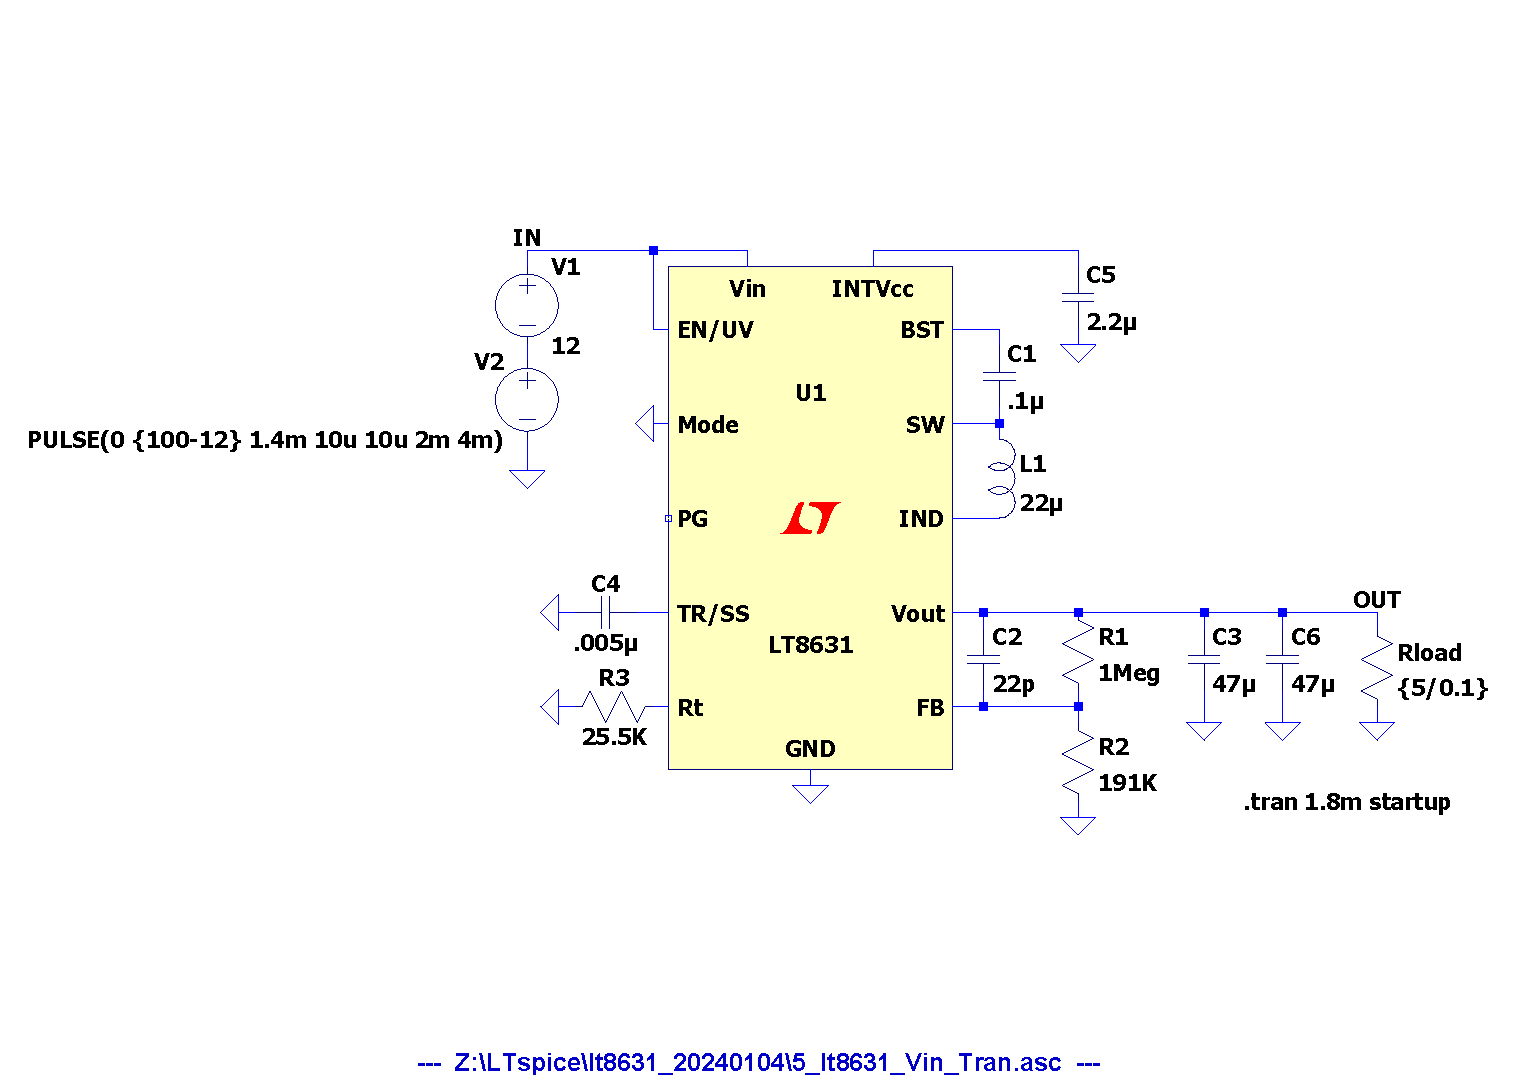
\includegraphics[page=1, width=0.6\textwidth]{figure/5_lt8631_Vin_Tran_asc.pdf}
    \caption{Input Voltage Transient Response}
\end{figure}

\subsection{运行结果}

运行得到下面的波形图。

\begin{figure}[htbp]
    \centering\begin{minipage}[t]{0.48\textwidth}
        \centering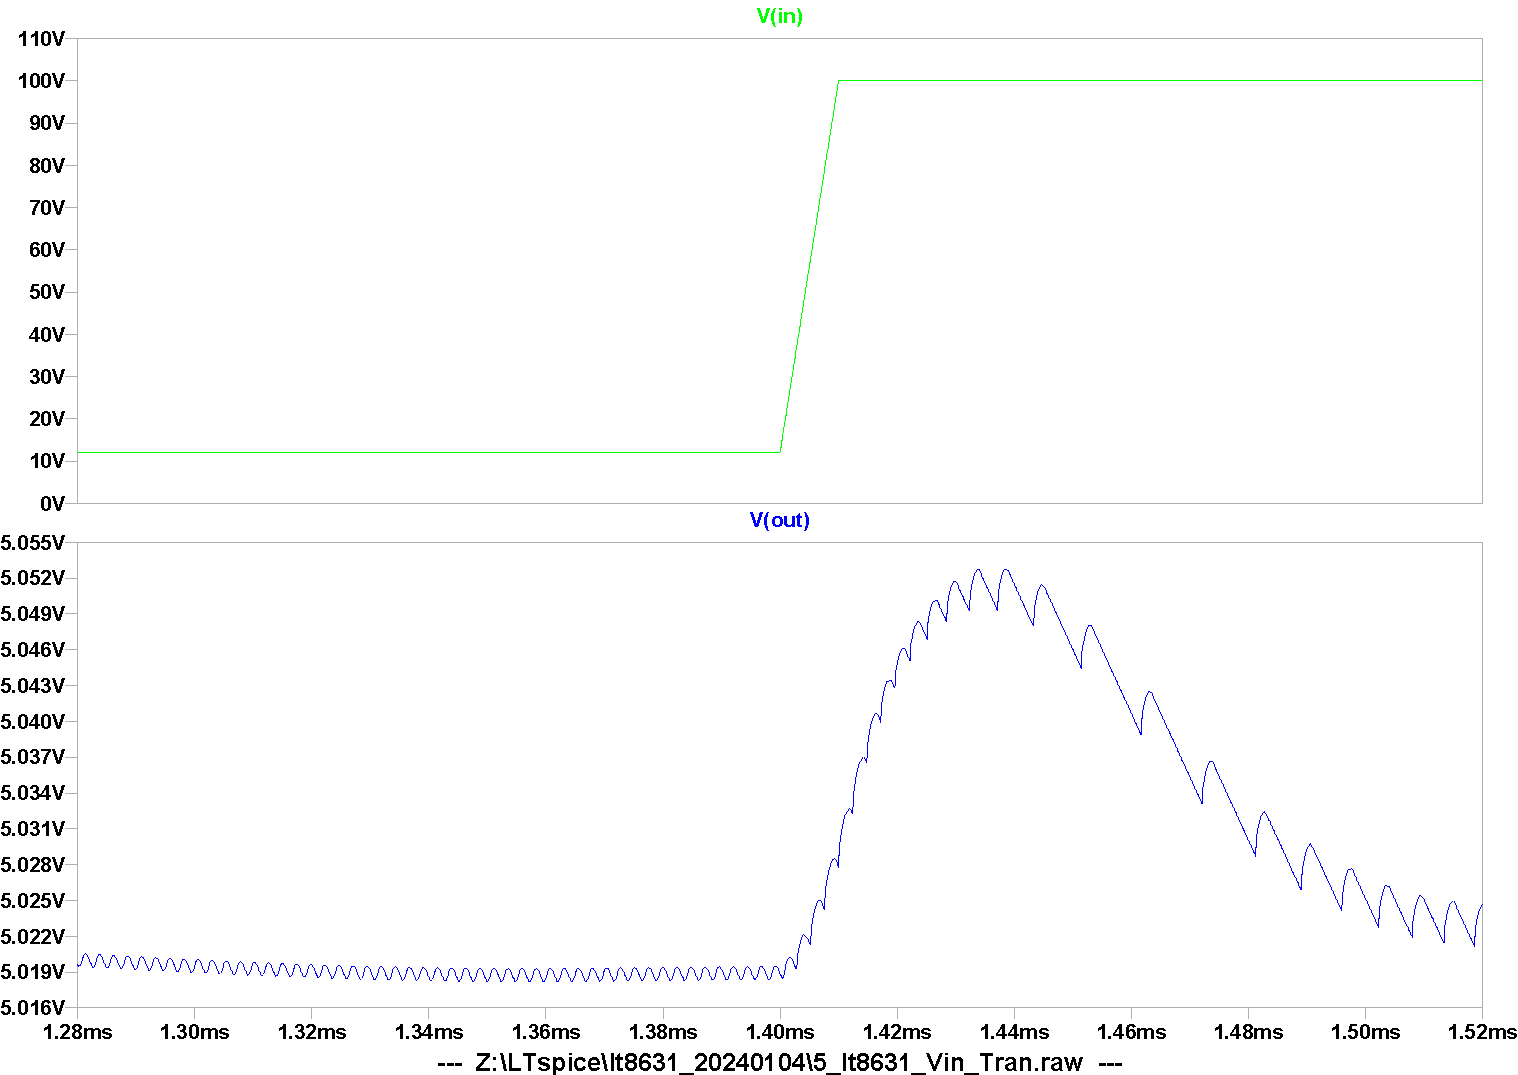
\includegraphics[page=1, width=0.9\textwidth]{figure/5_lt8631_Vin_Tran_2.pdf}
        \caption{Input Voltage Transient Response}
    \end{minipage}
    \centering\begin{minipage}[t]{0.48\textwidth}
        \centering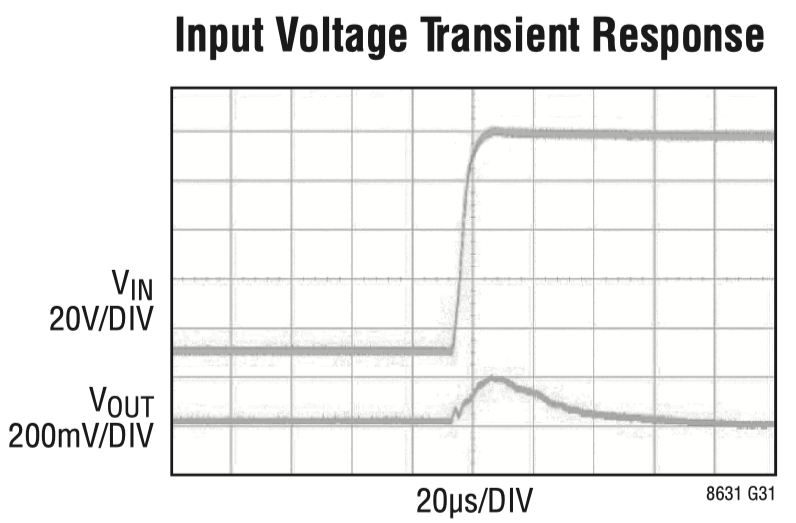
\includegraphics[width=0.9\linewidth]{figure/datasheet_G31.png}
        \caption{Input Voltage Transient Response}
    \end{minipage}
\end{figure}

\section{Start-Up Dropout Performance}

\subsection{任务详细内容}

满足以下条件下,仿真实现datasheet中的图32中所示 Start-Up Dropout Performance。

$I_{\text{LOAD}} = 500mA$

\subsection{功能描述}

% 请解释Start-Up Dropout Performance的含义。
% 请描述LT8631的datasheet中的Start-Up Dropout Performance的含义。

Start-Up Dropout Performance是指该电源转换器在输入电压低于输出电压时能否正常启动的性能。
如果输入电压高于最小的压差,该电源转换器可以维持输出电压,即使输入电压低于输出电压。
这种性能可以使该电源转换器在低压差或低输入电压的情况下工作,例如汽车的冷启动。
该电源转换器的最大占空比为99\%,这意味着它可以在极低的压差下工作。
Start-Up Dropout Performance可以通过测量输入电压和输出电压的波形来评估。

为了测试 Start-Up Dropout Performance,先建立下面的电路图。

\begin{figure}[!htb]
    \centering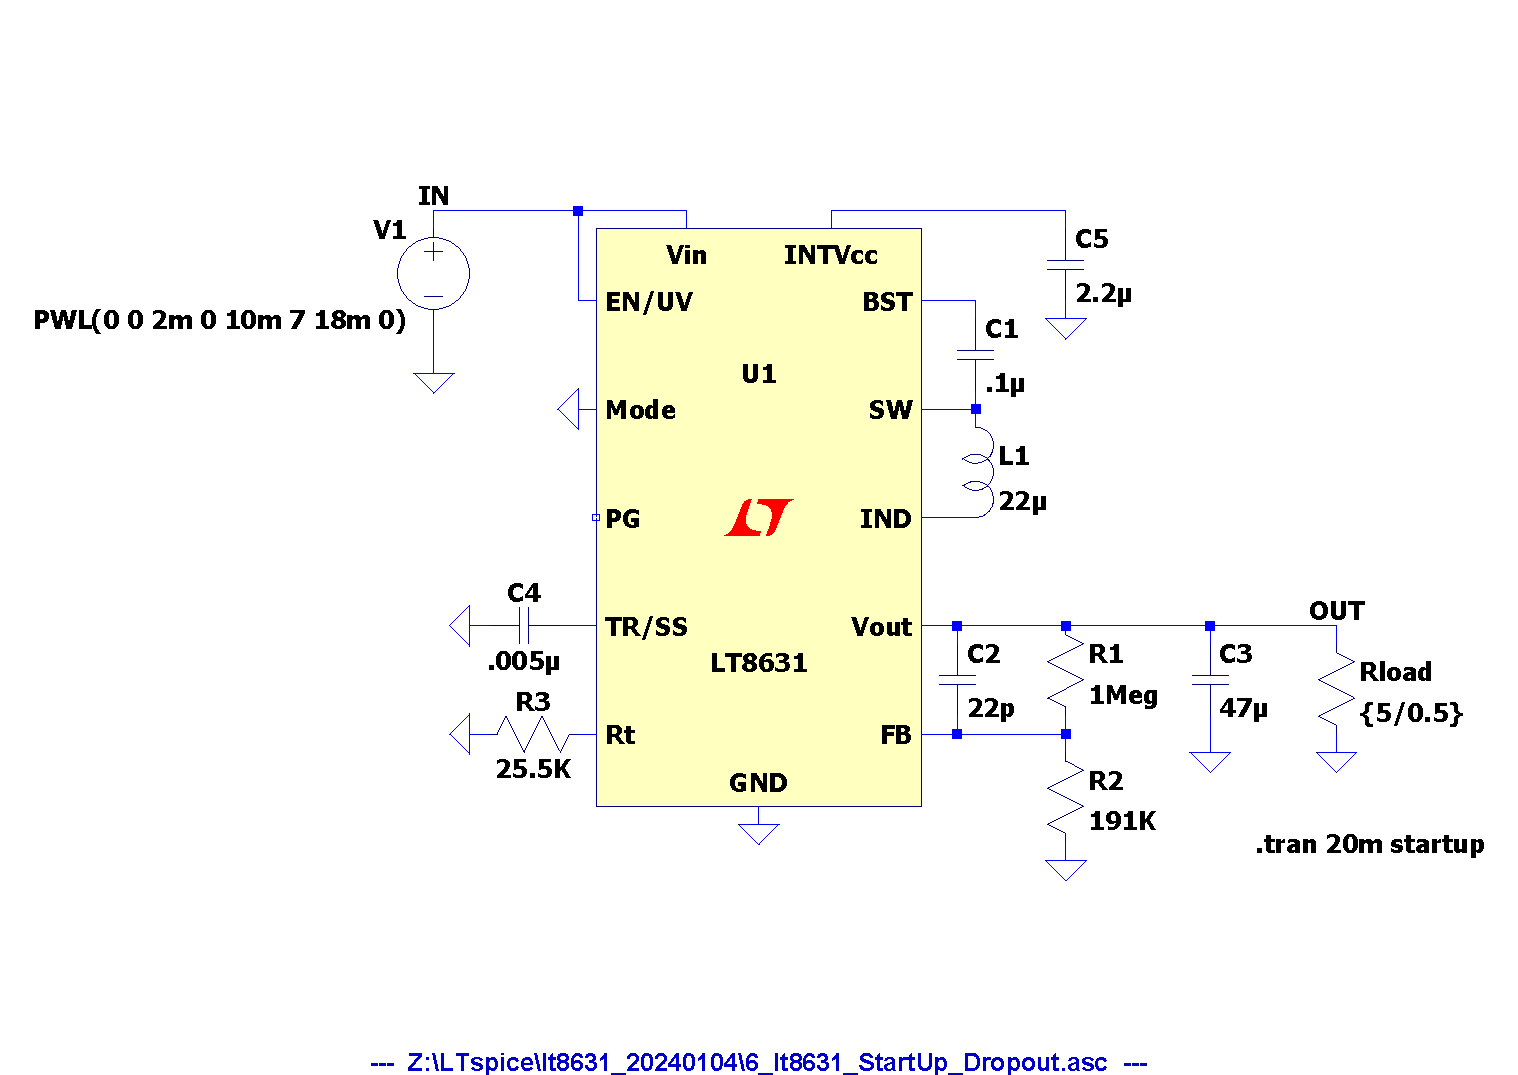
\includegraphics[page=1, width=0.6\textwidth]{figure/6_lt8631_StartUp_Dropout_asc.pdf}
    \caption{Start-Up Dropout Performance}
\end{figure}

\subsection{运行结果}

运行得到下面的波形图。

\begin{figure}[htbp]
    \centering\begin{minipage}[t]{0.48\textwidth}
        \centering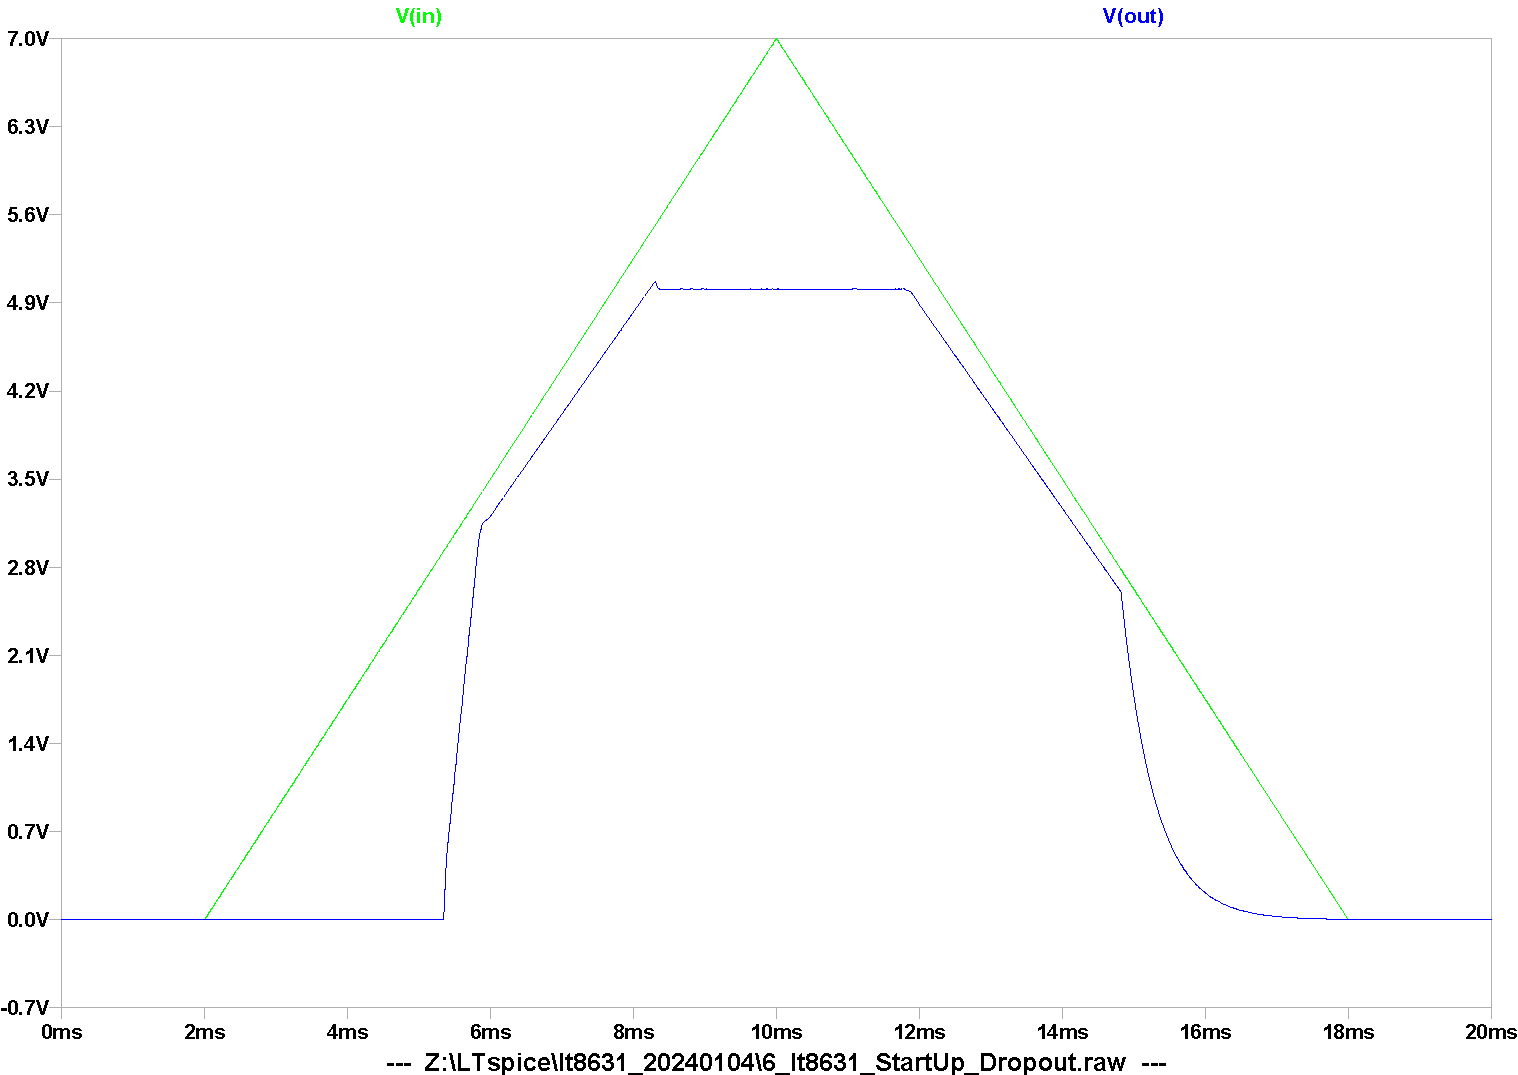
\includegraphics[page=1, width=0.9\textwidth]{figure/6_lt8631_StartUp_Dropout_1.pdf}
        \caption{Start-Up Dropout Performance}
    \end{minipage}
    \centering\begin{minipage}[t]{0.48\textwidth}
        \centering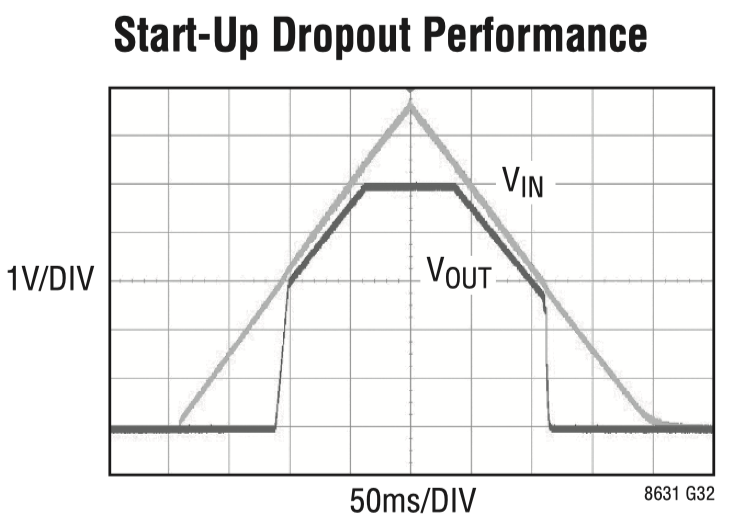
\includegraphics[width=0.9\linewidth]{figure/datasheet_G32.png}
        \caption{Start-Up Dropout Performance}
    \end{minipage}
\end{figure}

\chapter{论文总结}

本任务是使用LTspice对LT8631进行仿真分析的综合性实验,旨在学习LTspice的基本操作和应用,以及LT8631的主要性能参数和工作原理。
通过完成本任务,我深入了解LT8631的效率、突发模式、开关模式、负载瞬态响应、输入电压瞬态响应和启动失调电压等特性,以及它们与输入电压、输出电压、负载电流和开关频率等因素的关系。
本任务对于提高我的电路设计和仿真能力,以及培养我的创新思维和实践能力,具有重要的意义。

在本次任务仿真过程中,我发现了以下几个问题和困难,以及相应的解决方法:

\begin{itemize}
    \item LTspice中的波形查看器有时会出现缩放和标尺的问题,需要手动调整或使用快捷键来解决。
    \item LTspice中的突发模式和开关模式的切换需要根据datasheet中的公式,计算出合适的RT引脚的电阻值,并使用.STEP命令进行重复分析,得到不同模式下的波形图。
    \item LTspice中的负载瞬态和输入电压瞬态的模拟需要使用时间依赖的源,并设置其在一定范围内变化,然后使用.TRAN命令进行瞬态分析,得到输出电压的波形图。
    \item LTspice中的启动失调电压的模拟需要使用.PULSE命令,设置输入电压在一定时间内的变化,然后使用.TRAN命令进行瞬态分析,得到输出电压的波形图。
\end{itemize}


实验报告使用的是latex,这是一种优秀的文档排版系统,可以用来制作高质量的实验报告。在使用latex编写报告时,我学到了以下几点:

\begin{itemize}
    \item latex的基本结构是由导言区和正文区组成,导言区用来设置文档的类别、引用的宏包、自定义的命令等,正文区用来编写实际的内容。
    \item latex的优势之一是可以方便地插入图片,只需使用\textbackslash includegraphics命令,并指定图片的文件名、大小、位置等参数。图片的格式可以是eps、pdf、png、jpg等,但需要注意与编译方式的兼容性。
    \item latex还可以自动生成目录、编号、引用等,只需使用相应的命令,如cite等,并在编译时运行相应的程序,如latex、bibtex、xelatex等。
    \item latex的另一个优势是可以轻松地编写数学公式,只需使用数学模式,并使用各种数学符号和命令。
\end{itemize}

% \bibliographystyle{unsrt}
\bibliography{reference.bib}

% \nocite{*}
\newrefcontext[sorting=none]
\printbibliography[heading=bibintoc, title=\ebibname]
% \bibliography{ref}

\section{Reference}

[1] \href{https://www.analog.com/media/en/technical-documentation/data-sheets/lt8631.pdf}{LT8631 datasheet}.

\end{document}
